\documentclass[11pt,a4paper]{article}
\usepackage[margin=24mm]{geometry}
\usepackage{amsmath,amssymb,amsthm,mathtools,bm,booktabs,array,longtable}
\usepackage[T1]{fontenc}
\usepackage{lmodern,microtype,graphicx,xcolor,xurl,hyperref}
\hypersetup{colorlinks=true,linkcolor=blue!45!black,urlcolor=blue!45!black,citecolor=blue!45!black,pdftitle={The full correlation range, filtering frontier and volume trade-off at fixed steering centre},pdfauthor={Dev D. Goyal},pdfsubject={Exact F3 correlation intervals, probability-constrained filtering, steering-ellipsoid volume and Lean matrix proofs}}
\setlength{\parskip}{5pt}\setlength{\parindent}{0pt}
\widowpenalty=10000\clubpenalty=10000
\newtheorem{theorem}{Theorem}
\newtheorem{lemma}[theorem]{Lemma}
\newtheorem{corollary}[theorem]{Corollary}
\newtheorem{proposition}[theorem]{Proposition}
\theoremstyle{remark}\newtheorem{remark}[theorem]{Remark}
\newcommand{\Tr}{\operatorname{Tr}}
\newcommand{\tr}{\operatorname{tr}}
\newcommand{\Id}{\mathbb I}
\newcommand{\norm}[1]{\left\lVert#1\right\rVert}
\newcommand{\R}{\mathbb R}
\newcommand{\C}{\mathbb C}
\newcommand{\bs}{\boldsymbol\sigma}
\renewcommand{\aa}{\mathbf a}\newcommand{\bb}{\mathbf b}
\newcommand{\cc}{\mathbf c}\newcommand{\nn}{\mathbf n}
\newcommand{\yy}{\mathbf y}
\title{The full correlation range, filtering frontier and\\volume trade-off at fixed steering centre}
\author{Dev D. Goyal}
\date{3 November 2026}
\begin{document}
\maketitle
\begin{abstract}
For two-qubit states we study the three-setting correlation value
$F_3=\norm T_{\mathrm F}$ of Eq.~(3) of Ducuara, Susa and Skrzypczyk
(arXiv:2406.03945) as a function of the steering-ellipsoid geometry.
An earlier package in this collection determined the exact supremum
$G(c)$ of $F_3^2$ at fixed centre length $c$, with violation $F_3>1$
possible exactly when $c<2/3$. Here we determine the entire attainable
set at fixed centre length $c$ and Bob Bloch length $r<1$: it is the closed
interval
$\bigl[\max\{0,c(1+r)-1\}^2,\ (1-r^2)(3-4c)+(c+(1-c)r)^2\bigr]$, with
separable diagonal minimizers, a classification of the lower endpoint and
a trace-norm stability estimate. For canonical states with centre
length $c$ and radial support half-width $t$, the squared correlation
$\tau=\norm S_{\mathrm F}^2$ fills $[t^2,1-c^2+2t^2]$, and the greatest
ellipsoid volume at prescribed $(c,t,\tau)$ is
$(4\pi/3)(t/2)\min\{\tau-t^2,\,1+2t+2t^2-c^2-\tau\}$, attained at every
feasible triple. A canonical input and a Bob filter succeeding with
probability at least $p\in[1/2,1]$ can produce $F_3>1$ exactly when
$c<2/[1+p+\sqrt{(1-p)^2+2}]$. We also solve every one-sided filtering
orbit exactly, including singular hard cases, and classify the maximizers
of $G(c)$ with explicit trace-norm rigidity. Lean~4 with Mathlib proves the
central statements for actual complex $4\times4$ density matrices, Kraus
operators and local unitaries; the remaining statements, listed in
Appendix~\ref{sec:verification}, have conventional proofs.
\end{abstract}

\section{Introduction}
Ducuara, Susa and Skrzypczyk~\cite{ducuara} relate hidden steering to the
steering ellipsoid of Jevtic, Pusey, Jennings and Rudolph~\cite{jevtic}.
They leave open the function bounding the three-setting correlation
value $F_3=\norm T_{\mathrm F}$ in terms of the centre length $c$ of Alice's
steering ellipsoid, and report from random states an apparent cutoff near
$c\approx0.66$ for violation of $F_3\leq1$. An earlier package in this
collection, \emph{Exact three-setting correlation bounds at fixed steering
centre}~\cite{earlier}, dated 29 October 2026, answered that question: it
proved that the least upper bound of $F_3^2$ at centre length $c$ is
$G(c)=1+(2-3c)^2/(2-2c-c^2)$ for $c\leq2/3$ and $1$ for $c>2/3$, attained
exactly for $c<2/3$ and $c=1$, together with the joint upper bound
$F_3^2\leq H_c(r)$ at Bob Bloch length $r$ and its attainment along one
explicit family. This paper determines the remaining parts of the picture.

\paragraph{The question and the answers in plain terms.} In Bloch form a
two-qubit state has three ingredients: Alice's local vector $\aa$, Bob's local
vector $\bb$, and the $3\times3$ matrix $T$ of correlations between spin
measurements on the two qubits. The number $F_3=\norm T_{\mathrm F}$ measures
how strongly the spins are correlated along three orthogonal measurement
directions; a value above one violates the corresponding three-setting
steering inequality. Alice's steering ellipsoid is the set of Bloch vectors
to which Bob's measurements can steer Alice's qubit, and its centre and shape
constrain $T$. The earlier package found the largest $F_3$ compatible with a
given centre length. This paper answers three follow-up questions.
\begin{itemize}
\item \emph{Which values of $F_3$ are possible once both the centre length and
the length $r$ of Bob's Bloch vector are fixed?} Exactly an interval. Its new
lower end says that a long centre together with a strongly polarized Bob forces
some correlation, because otherwise the probability of one particular pair of
measurement outcomes would be negative.
\item \emph{When can a local filter on Bob's side, required to succeed with
probability at least $p$, reveal a hidden violation?} Exactly when the centre
length lies below an explicit threshold, which decreases from $2/3$ at $p=1/2$
to $2-\sqrt2$ at $p=1$.
\item \emph{How large can the steering ellipsoid be when its correlation
strength is fixed?} At most an explicit piecewise linear cap in the squared
correlation, attained everywhere. The states with the largest correlation do
not have the largest volume: the two objectives compete for the same
off-diagonal entries of the density matrix.
\end{itemize}

\paragraph{Main results.} For centre length $c\in[0,1]$ and Bob Bloch
length $r\in[0,1)$:
\begin{enumerate}
\item The set of attainable values of $F_3^2$ is exactly the interval
$[L(c,r),H_c(r)]$, $L(c,r)=\max\{0,c(1+r)-1\}^2$,
$H_c(r)=(1-r^2)(3-4c)+(c+(1-c)r)^2$ (Theorem~\ref{thm:jointrange}).
The lower endpoint has separable diagonal witnesses, every minimizer is
locally unitarily equivalent to the witness, and a state with
$F_3^2=L(c,r)+\eta$ lies within squared trace norm $(1+r^2)\eta$ of an
explicit minimizer. At $r=1$ the only value is $c^2$.
\item For canonical states (Bob maximally mixed) with centre $c\nn$ and
radial support half-width $t=\norm{S^{\mathsf T}\nn}$, the attainable
squared correlations form $[t^2,1-c^2+2t^2]$, for exactly
$0\leq t\leq 1-c$ (Theorem~\ref{thm:canonical-interval-v2}); the signed
determinant fills $[-t((1+t)^2-c^2)/4,\ t((1-t)^2-c^2)/4]$; and at
prescribed $(c,t,\tau)$ the greatest $|\det S|$ is
$(t/2)\min\{\tau-t^2,1+2t+2t^2-c^2-\tau\}$, attained at every feasible
triple (Theorems~\ref{thm:volume-radial-v2} and~\ref{thm:triple-volume-v2}).
The ellipsoid volume is $(4\pi/3)|\det S|$. At $t=1-c$ this recovers the
fixed-centre volume maximum $(4\pi/3)(1-c)^2$ of Milne
et~al.~\cite{milnevolume}.
\item Over canonical inputs of centre length $c$ and Bob Kraus operators
with success probability at least $p\in[1/2,1]$, the greatest $F_3^2$ of
the normalized output is $H_c(\widehat r)$ with $\widehat r$ the clipped
vertex of $H_c$ on $[0,(1-p)/p]$, and violation is possible exactly when
$c<2/[1+p+\sqrt{(1-p)^2+2}]$ (Theorem~\ref{thm:probability-envelope-v2}
and Corollary~\ref{cor:success-threshold-v2}).
\item Every one-sided filtering orbit of a canonical state is solved by an
explicit spectral algorithm with at most seven algebraic candidates,
including singular and hard cases, with all maximizing effects classified
(Sections~\ref{sec:orbit} and~\ref{sec:complete-trust-region}).
\item The maximizers of $G(c)$ are classified up to local unitaries, with
explicit trace-norm stability of the canonical optimizer
(Theorems~\ref{thm:classification} and~\ref{thm:stability},
Appendix~\ref{sec:matrix-rigidity}).
\end{enumerate}

\paragraph{What is new, and what is not.} The envelope $G(c)$, the
threshold $c<2/3$, the joint upper bound $H_c(r)$ with its attaining
family, and the fully entangled fraction bound are results of the earlier
package~\cite{earlier}; Sections~\ref{sec:global} and~\ref{sec:witness}
recall them so that this paper is self-contained. New relative to that
package are the lower bound $L(c,r)$ and the complete joint interval, the
lower-endpoint classification and stability, the canonical $(c,t)$
interval, the probability-constrained frontier, the complete solution of
the one-sided filtering orbits, the classification and trace-norm rigidity
of the maximizers, the flat-branch stability exponents, and the signed and
three-parameter volume bounds. Classical ingredients are credited where
they are used: the steering-ellipsoid and canonical-filtering framework
and the maximally obese states~\cite{jevtic,milne,milnevolume}, the
spin-flip method and Bloch-matrix positivity~\cite{milne,jevtic,gamel},
the measurement optimization behind the interpretation of
$F_3$~\cite{costa}, marginal spectral constraints~\cite{bravyi}, and
trust-region theory for quadratics on a ball~\cite{more,fortin}.
The fixed-centre volume maximum is Theorem~3 of~\cite{milnevolume}.
A bounded literature search did not find the new frontiers; this does not
establish priority.

\paragraph{Earlier public record.} On 31 October 2026 a check of public
records found that the Omega Institute's public repository records a
claimed Lean proof of Conjecture~2 of Milne, Jennings, Jevtic and
Rudolph~\cite{milne}, the fully entangled fraction bound $f\leq1-c/2$ at
fixed centre, committed on 8 October 2026 (issue \#14206)~\cite{omegafef},
and a proof of their Conjecture~1, a sharp bound on the CHSH value at fixed
centre, committed on 14 October 2026 (issue \#16558)~\cite{omegachsh}.
The Lean project of this package contains, unchanged from the earlier
package, a proof of the fully entangled fraction bound; no priority is
claimed for it, and it is not a result of this paper. The CHSH value is a
different quantity from $F_3$. The CHSH dossier also records, as an
intermediate lemma proved with the same filtering covariance identity, an
upper bound on the CHSH value in terms of both $c$ and Bob's Bloch length;
it lists the $F_3$ centre bound as open. As read on 3 November 2026,
neither dossier treats the lower bound or the full interval of $F_3^2$, the
probability frontier, the filtering orbits or the volume bounds.
Xing and Yang~\cite{xing} give volume-based bounds on entanglement and Bell
nonlocality through the steering ellipsoid; their full text was not
compared with this paper.

\paragraph{Verification.} Lean~4.19.0 with Mathlib proves the joint
interval, the lower-endpoint equality and trace-norm rigidity, the
canonical $(c,t)$ interval, the probability frontier from actual Kraus
operators, the complete orbit solution, the classification and rigidity of
the maximizers, and the signed and three-parameter volume maxima, for
actual complex density matrices; a whole-project audit confirms that every
declaration other than compiler-generated auxiliaries depends only on the
standard axioms. The flat-branch
exponents, the volume-maximizer orbit classification and rank counts, the
attainment of every signed determinant, and the physical interpretation of
$F_3$ rest on conventional proofs. Appendix~\ref{sec:verification} gives
the details.

\paragraph{Organization.} Section~\ref{sec:defs} fixes notation.
Section~\ref{sec:geometric} proves a rank-safe geometric inequality and the
sharp centre and radial-width envelope, and Section~\ref{sec:global} recalls
the envelope of the earlier package; everything else builds on these.
Sections~\ref{sec:jointrange}--\ref{sec:volume-v2} contain the new joint
interval, the canonical interval with the probability frontier, and the
volume bounds. Sections~\ref{sec:classification}--\ref{sec:complete-trust-region}
classify the maximizers, quantify their stability and solve the one-sided
filtering orbits. Section~\ref{sec:scope} states the scope. The appendices
give the matrix proofs of rigidity (Appendix~\ref{sec:matrix-rigidity}), the
comparison with the earlier package (Appendix~\ref{sec:audit}) and the
verification record (Appendix~\ref{sec:verification}).

\section{Definitions and conventions}\label{sec:defs}
Write an arbitrary two-qubit density matrix as
\begin{equation}\label{eq:bloch}
\rho=\frac14\left(\Id\otimes\Id+\aa\cdot\bs\otimes\Id
+\Id\otimes\bb\cdot\bs+\sum_{i,j=1}^3T_{ij}\sigma_i\otimes\sigma_j\right),
\qquad \rho\succeq0,\quad\Tr\rho=1.
\end{equation}
The correlation quantity in Eq.~(3) of Ducuara--Susa--Skrzypczyk~\cite{ducuara}
is $F_3(\rho)=\norm T_F$, with violation when $F_3>1$. Its identification with
the optimized three-setting linear CJWR expression uses the measurement
optimization of Costa--Angelo~\cite{costa}. This is a particular steering
inequality; $F_3\leq1$ does not prove the existence of a local hidden-state
model for all measurements.
The orthonormal Bob triad is optimized here. If that triad is fixed and only
Alice's three directions are optimized, the value is instead
$\sum_j\norm{T\mathbf e_j}/\sqrt3$, which can be smaller than $\norm T_F$.
Thus the matrix target is exactly the convention of Eq.~(3), not an
assertion about every fixed laboratory frame.

We use Alice's steering ellipsoid. Put $r=\norm\bb$. If $r<1$, its centre is
\begin{equation}\label{eq:center}
\cc=\frac{\aa-T\bb}{1-r^2},\qquad c=\norm\cc.
\end{equation}
Whitening Bob produces the canonical state
\begin{equation}\label{eq:white}
\sigma=(\Id\otimes(2\rho_B)^{-1/2})\rho(\Id\otimes(2\rho_B)^{-1/2}),
\qquad \sigma_B=\Id/2.
\end{equation}
Its Alice Bloch vector is $\cc$; write its correlation matrix as $S$ and its
ellipsoid matrix as $Q=SS^{\mathsf T}$. These conventions are standard in the
steering-ellipsoid construction~\cite{jevtic,milne}. Swapping Alice and Bob
gives an identical theorem for the other centre.

If $r=1$, the state is a product $\rho_A\otimes|\beta\rangle\langle\beta|$.
Its steering set is one point; we define its centre to be $\aa$. This is a
separate case, not a substitution into the zero denominator in
\eqref{eq:center}.

The 2024 paper leaves the function bounding $F_3$ in terms of $c$ undetermined
and reports an apparent cutoff near $0.66$ from random states. The earlier
package~\cite{earlier} showed that the exact threshold is $2/3$;
Section~\ref{sec:witness} recalls an exact state with centre length above
$0.66$ and $F_3>1$.

\section{A rank-safe geometric inequality}\label{sec:geometric}
The following supplies an independent geometric route to the canonical bound
used by the earlier proof. It is stronger than a bound involving $c$ alone.

\begin{theorem}[Directional matrix inequality]\label{thm:lmi}
For every state \eqref{eq:bloch}, without a rank restriction,
\begin{align}
M_A&=(1+\norm\aa^2-\norm\bb^2-\norm T_F^2)\Id_3
+2(TT^{\mathsf T}-\aa\aa^{\mathsf T})\succeq0,\label{eq:lmi}\\
M_B&=(1+\norm\bb^2-\norm\aa^2-\norm T_F^2)\Id_3
+2(T^{\mathsf T}T-\bb\bb^{\mathsf T})\succeq0.
\end{align}
For a unit vector $\nn$, equality $\nn^{\mathsf T}M_A\nn=0$ holds exactly when
$\rho$ and the positive spin-flipped state defined below have orthogonal supports.
\end{theorem}
\begin{proof}
Let $Y=\sigma_y$, $N=\nn\cdot\bs$, and define
\[
\widetilde\rho=(Y\otimes Y)\overline\rho(Y\otimes Y),\qquad
\rho_{\nn}=(N\otimes\Id)\widetilde\rho(N\otimes\Id).
\]
Complex conjugation preserves positivity. Both conjugating matrices are
unitary for unit $\nn$, so $\rho_{\nn}\succeq0$. The full spin flip sends
$(\aa,\bb,T)$ to $(-\aa,-\bb,T)$, and conjugation by $N$ acts on Alice's
Bloch space by $R_{\nn}=2\nn\nn^{\mathsf T}-\Id$. Pauli orthogonality gives
the exact identity
\begin{equation}\label{eq:overlap}
4\Tr(\rho\rho_{\nn})=1+\norm\aa^2-\norm\bb^2
-2(\aa\cdot\nn)^2+2\norm{T^{\mathsf T}\nn}^2-\norm T_F^2
=\nn^{\mathsf T}M_A\nn.
\end{equation}
The left side is nonnegative because it is the trace of
$\rho^{1/2}\rho_{\nn}\rho^{1/2}\succeq0$. Homogeneity extends nonnegativity
from unit vectors to all real vectors. Exchange the two qubits for $M_B$.

If the overlap is zero, the positive matrix
$\rho^{1/2}\rho_{\nn}\rho^{1/2}$ is zero. Equivalently,
$\rho_{\nn}^{1/2}\rho^{1/2}=0$, giving orthogonal supports and
$\rho\rho_{\nn}=0$. The converse is immediate. No inverse is used.
\end{proof}

\begin{theorem}[Sharp centre and radial-width envelope]\label{thm:radial}
For a canonical state with centre $\cc$, choose $\nn=\cc/c$ when $c>0$;
when $c=0$, choose any unit direction. Put
\[
t=\norm{S^{\mathsf T}\nn},\qquad q=t^2=\nn^{\mathsf T}Q\nn.
\]
Then
\begin{equation}\label{eq:radial}
0\leq t\leq1-c,\qquad \tr Q\leq1-c^2+2t^2.
\end{equation}
For every $0\leq c\leq1$ and $0\leq t\leq1-c$, the upper bound is attained.
Consequently, if
$\delta=(1-c)(3-c)-\tr Q$, then
\begin{equation}\label{eq:radialgap}
\delta\geq2\big((1-c)^2-q\big)\geq0.
\end{equation}
\end{theorem}
Here $t$ is the support half-width of the ellipsoid in the centre direction.
For a tilted ellipsoid it need not be a semiaxis or its radius along that ray.

\begin{proof}
Specialize \eqref{eq:lmi} to $\bb=0$, $\aa=\cc$, and evaluate it on $\nn$.
This gives the second inequality in \eqref{eq:radial}.
Every conditional Bloch vector $\cc+S\mathbf u$, $\norm{\mathbf u}\leq1$,
has norm at most one. Maximizing its projection on $\nn$ gives
$c+\norm{S^{\mathsf T}\nn}=c+t\leq1$. This argument is valid also at $t=0$.
Substitute $t\leq1-c$ to obtain \eqref{eq:radialgap}.

For sharpness, define
\[
a_\pm=\frac{1+c\pm t}{4},\qquad d_\pm=\frac{1-c\pm t}{4},\qquad
w=\sqrt{a_+d_+},\quad v=\sqrt{a_-d_-},
\]
and, in the order $00,01,10,11$, set
\begin{equation}\label{eq:radialwitness}
\sigma_{c,t}=\begin{pmatrix}
a_+&0&0&w\\0&a_-&v&0\\0&v&d_-&0\\w&0&0&d_+
\end{pmatrix}.
\end{equation}
All four diagonal parameters are nonnegative. After grouping the pairs
$00,11$ and $01,10$, the matrix is the direct sum of two positive matrices of
rank at most one, including a zero block at an endpoint. Its eigenvalues are
$(1+t)/2,(1-t)/2,0,0$.
Its marginals are $(\Id+cZ)/2$ and $\Id/2$, and
\[
S=\operatorname{diag}(2(w+v),2(v-w),t).
\]
Hence $\norm{S^{\mathsf T}\mathbf e_z}^2=t^2$ and
$\tr Q=8(w^2+v^2)+t^2=1-c^2+2t^2$. The construction includes the zero-block
endpoints, the rank-one Bell state $(c,t)=(0,1)$, and the product
$|0\rangle\langle0|\otimes\Id/2$ at $(1,0)$.
\end{proof}

\section{The exact global correlation envelope}\label{sec:global}
The envelope, the joint upper bound and the attaining family in this
section are results of the earlier package~\cite{earlier}. We recall them
with their proofs, because the new results build on the same identities.

\begin{lemma}[Exact filter identity and marginal bound]\label{lem:filter}
Let $\sigma_B=\Id/2$, and let $F\succeq0$ satisfy $\Tr F^2=2$.
Write $\rho=(\Id\otimes F)\sigma(\Id\otimes F)$ and $r=\norm\bb$. Then
\begin{align}
\norm T_F^2&=(1-r^2)(\norm S_F^2-c^2)+\norm\aa^2,\label{eq:filteridentity}\\
\norm\aa&\leq c+(1-c)r.\label{eq:marginal}
\end{align}
These identities and inequalities remain valid for singular $F$ when $c$
means the prefilter canonical centre.
\end{lemma}
\begin{proof}
For any complex $4\times4$ matrix $X$, define
$E(X)=\Tr(X^2)-\Tr((\Tr_BX)^2)$. For every $2\times2$ matrix $F$,
\begin{equation}\label{eq:detcov}
E((\Id\otimes F)X(\Id\otimes F))=\det(F)^2E(X).
\end{equation}
To verify this, write $X$ in Bob-valued blocks $X_{ij}$ and use
$E(X)=\sum_{ij}[\Tr(X_{ij}X_{ji})-\Tr X_{ij}\Tr X_{ji}]$.
Polarizing the $2\times2$ determinant identity under $A\mapsto FAF$ proves
the equality for each pair of blocks. It is a polynomial identity and
requires neither an inverse nor positivity.

Here $\rho_B=F^2/2$, so $\det(F)^2=1-r^2$.
The Pauli purity identity
$4\Tr\rho^2=1+\norm\aa^2+\norm\bb^2+\norm T_F^2$
turns \eqref{eq:detcov} into \eqref{eq:filteridentity}.

The smallest eigenvalue of $F^2$ is $1-r$, so
$K=F^2-(1-r)\Id\succeq0$ and $\Tr K=2r$. Put
$R=\Tr_B[\sigma(\Id\otimes K)]$. Partial-trace cyclicity writes $R$ as the
partial trace of a positive congruence, proving $R\succeq0$. Moreover
$\Tr R=r$ and $\rho_A=(1-r)\sigma_A+R$.
The Bloch-vector length of a positive qubit matrix is bounded by its trace.
The triangle inequality therefore gives \eqref{eq:marginal}, including $r=0,1$.

For the centre identification, let $B=\bb\cdot\bs=F^2-\Id$.
The filter commutes with $B$, and $B^2=r^2\Id$, so
$FBF=B+r^2\Id$. Taking Pauli expectations and using partial-trace cyclicity
gives
\[
\aa=\cc+S\bb,\qquad T\bb=S\bb+r^2\cc,\qquad
\aa-T\bb=(1-r^2)\cc.
\]
For $r<1$ this proves that the whitening centre is exactly
\eqref{eq:center}. It requires no inverse of the joint state.
\end{proof}

\begin{theorem}[Joint bound and global envelope]\label{thm:global}
For an actual output state with $r<1$ and centre length $c$,
\begin{equation}\label{eq:joint}
F_3(\rho)^2\leq H_c(r):=(1-r^2)(3-4c)+[c+(1-c)r]^2.
\end{equation}
For every pair $0\leq c\leq1$, $0\leq r<1$, equality is attained. At $r=1$
the sharp bound at the actual output centre is instead $c^2$.

Over all states with specified actual centre length $c$,
\begin{equation}\label{eq:global}
\sup F_3^2=G(c)=\begin{cases}
1+\dfrac{(2-3c)^2}{2-2c-c^2},&0\leq c<2/3,\\[5pt]
1,&2/3\leq c\leq1.
\end{cases}
\end{equation}
The supremum is attained for $c<2/3$ and $c=1$, and is not attained for
$2/3\leq c<1$. There exists an $F_3$-violating state at centre length $c$
if and only if $c<2/3$.
\end{theorem}
\begin{proof}
For $r<1$, use \eqref{eq:white} and apply Theorem~\ref{thm:radial} and
Lemma~\ref{lem:filter}. They give
$\norm S_F^2-c^2\leq3-4c$ and \eqref{eq:joint}.

Put $d=1-c$ and $D(c)=2-2c-c^2$. Then
$H_c(r)=3-4c+c^2+2cd\,r-D(c)r^2$. On $0\leq c\leq2/3$, $D(c)>0$ and
\begin{equation}\label{eq:square}
G(c)-H_c(r)=D(c)\left(r-\frac{c(1-c)}{D(c)}\right)^2.
\end{equation}
The optimizer $r_*=c(1-c)/D(c)$ belongs to $[0,1)$ exactly when $c<2/3$.
At $c=2/3$ it equals one. For $2/3\leq c\leq1$ the exact identity
\begin{equation}\label{eq:flat}
1-H_c(r)=(1-r)^2(4c-2-c^2)+r(1-r)(6c-4)
\end{equation}
is nonnegative. Its first coefficient is strictly positive throughout that
interval; thus $H_c(r)<1$ if $r<1$.

If $r=1$, positivity and the pure Bob marginal force the product form:
indeed the compression of $\rho$ to Bob's orthogonal marginal support has
trace zero, hence is zero, and positivity annihilates its off-support rows
and columns. Then $T=\aa\bb^{\mathsf T}$ and
$F_3^2=\norm\aa^2=c^2$. No extra maximizer appears when $c<1$.

The explicit family in the next subsection attains \eqref{eq:joint} for
every $r<1$. Choosing $r=r_*$ proves attainment on the first branch.
Letting $r\uparrow1$ proves sharpness of the flat branch. At $c=1$, a pure
product state attains one. Finally $G(c)>1$ precisely when $c<2/3$.
\end{proof}

\subsection{Explicit sharp states and exact counterexamples}\label{sec:witness}
The following family is a Bob-filtered maximally obese canonical state:
\begin{equation}\label{eq:globalwitness}
\rho_{c,r}=\frac12\begin{pmatrix}
1+r&0&0&\sqrt{(1-c)(1-r^2)}\\
0&c(1-r)&0&0\\
0&0&0&0\\
\sqrt{(1-c)(1-r^2)}&0&0&(1-c)(1-r)
\end{pmatrix},\quad 0\leq r<1.
\end{equation}
It is positive semidefinite and trace one. Its Bloch data are
\[
\aa=[c+(1-c)r]\mathbf e_z,\quad\bb=r\mathbf e_z,\quad
T=\operatorname{diag}\left(\sqrt{(1-c)(1-r^2)},-\sqrt{(1-c)(1-r^2)},1-c+cr\right).
\]
Substitution into \eqref{eq:center} gives $\cc=c\mathbf e_z$ and
$F_3^2=H_c(r)$. The canonical representative is $\sigma_{c,1-c}$.

At $c=3/5$ the best filter is $r=6/11$, giving
\[
\rho=\frac1{22}\begin{pmatrix}17&0&0&\sqrt{34}\\0&3&0&0\\0&0&0&0\\\sqrt{34}&0&0&2\end{pmatrix},
\qquad F_3^2=\frac{12}{11}>1.
\]
Its canonical representative has $F_3^2=24/25<1$. This explicitly excludes
the tempting but invalid argument that canonical filtering preserves $F_3$.

At $c=53/80=0.6625>0.66$, the exact optimizer is
$r=1431/1511$ and $F_3^2=1512/1511>1$. Thus the reported decimal $0.66$
can only be interpreted as numerical evidence near the true cutoff.

For $2/3\leq c<1$, the states \eqref{eq:globalwitness} approach
$|00\rangle\langle00|$ as $r\uparrow1$. That limit has centre length one,
not $c$. The fixed-$c$ set is not closed at this singular marginal boundary;
this explains why compactness of the entire density-matrix set does not
turn the supremum into a maximum.

\begin{figure}[ht]
\centering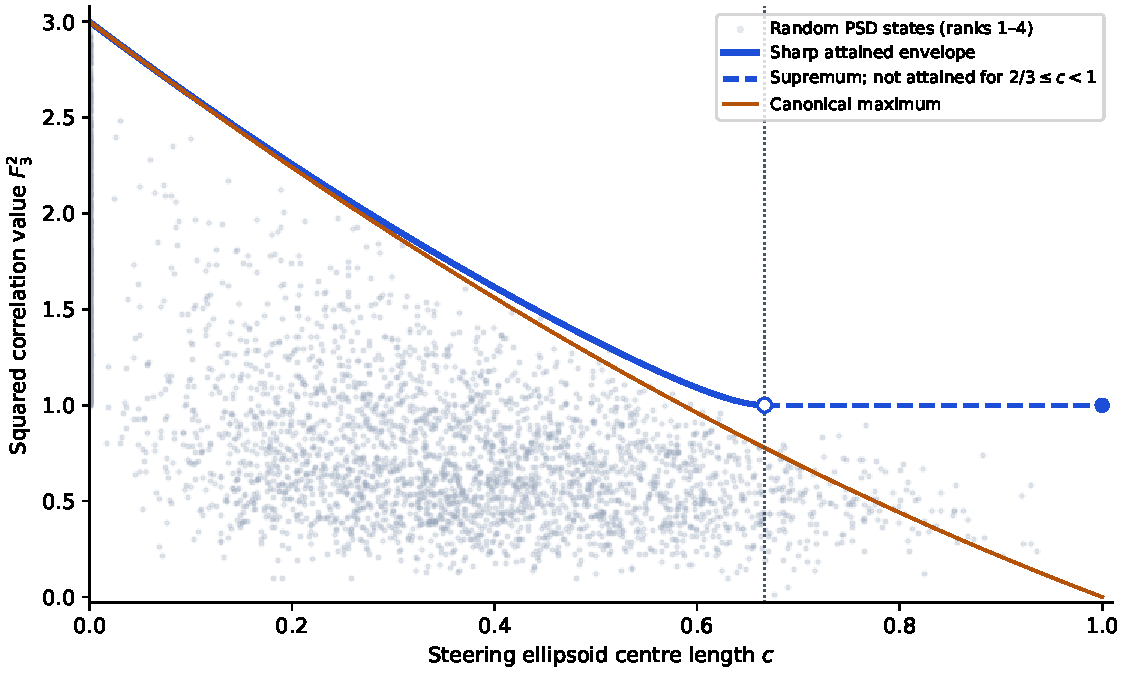
\includegraphics[width=.96\linewidth]{figures/envelope.pdf}
\caption{The exact envelope, with random states shown only as numerical
diagnostics. The dashed branch is not attained before $c=1$. Random sampling
is especially insensitive to the narrow violation region near $2/3$.}
\end{figure}

\section{The full correlation range at fixed centre and marginal}
\label{sec:jointrange}
The upper envelope has a complementary sharp lower bound. Together they
determine every possible value of the correlation norm, not merely its
largest value. This also identifies a region in which a nonzero centre
forces a strictly positive measured correlation.

\begin{theorem}[Complete joint range]\label{thm:jointrange}
Fix $0\leq c\leq1$ and $0\leq r<1$. Among all two-qubit density matrices
with Alice steering-centre length $c$ and Bob Bloch length $r$, the set of
attainable squared correlations is exactly
\begin{equation}\label{eq:jointinterval}
\left[\bigl(\max\{0,c(1+r)-1\}\bigr)^2,\;
 (1-r^2)(3-4c)+\bigl(c+(1-c)r\bigr)^2\right].
\end{equation}
Both endpoints are attained. The lower endpoint is attained by a state
diagonal in a product basis. Every lower-endpoint state is locally unitarily
equivalent to the displayed diagonal witness below. At $r=1$, the entire
range is instead the singleton $\{c^2\}$.
\end{theorem}

\begin{proof}
Choose unit vectors $\nn,\mathbf m$ so that the centre is $c\nn$ and
$\bb=r\mathbf m$. When a vector vanishes, choose its direction arbitrarily;
the argument does not divide by $c$ or $r$. Put
$q=\nn^{\mathsf T}T\mathbf m$. The probability of obtaining both minus
outcomes in the corresponding local spin measurements is nonnegative:
\[
 1-\aa\cdot\nn-r+q\geq0.
\]
The centre relation gives
$\aa\cdot\nn=(1-r^2)c+rq$, hence
\begin{equation}\label{eq:lowerfactor}
0\leq(1-r)\bigl(q-[c(1+r)-1]\bigr).
\end{equation}
Since $r<1$, $q\geq c(1+r)-1$. Cauchy--Schwarz gives
$|q|\leq\norm T_F$, proving the lower bound. The upper bound is the sharp
joint envelope proved earlier.

For attainment, put
\[
x=\max\{0,c(1+r)-1\},\qquad a_0=c(1-r^2)+rx.
\]
Take $\aa=a_0\mathbf e_z$, $\bb=r\mathbf e_z$, and
$T=\operatorname{diag}(0,0,x)$. The associated density matrix is
\begin{equation}\label{eq:jointlowerwitness}
\rho^-_{c,r}=\frac14\operatorname{diag}
 (1+a_0+r+x,\;1+a_0-r-x,\;1-a_0+r-x,\;1-a_0-r+x).
\end{equation}
If $x=0$, then $0\leq a_0\leq1-r$, so all entries are nonnegative.
If $x>0$, then $0<x\leq r$, $a_0=1-r+x$, and its eigenvalues are
\[
\frac{1+x}{2},\quad\frac{1-r}{2},\quad\frac{r-x}{2},\quad0.
\]
Its centre is exactly $c\mathbf e_z$ and $F_3^2=x^2$.
These checks include all vanishing diagonal entries, without assuming a
strictly positive state.

Let $\rho^+_{c,r}$ be the upper witness in
Eq.~\eqref{eq:globalwitness}, in the same coordinate convention.
Both witnesses have the same $\bb=r\mathbf e_z$ and the same vector
$\aa-T\bb=(1-r^2)c\mathbf e_z$. Every convex combination
\[
\rho_\alpha=(1-\alpha)\rho^-_{c,r}+\alpha\rho^+_{c,r},
\qquad0\leq\alpha\leq1,
\]
therefore has the same centre and Bob marginal. Write $d=1-c$ and
$z=d+cr$. Direct computation gives
\begin{equation}\label{eq:jointinterpolate}
F_3(\rho_\alpha)^2=
2\alpha^2d(1-r^2)+\bigl[x+\alpha(z-x)\bigr]^2.
\end{equation}
Here $x\geq0$ and $z-x\geq0$; for $x>0$, the latter difference is
$2(1-c)$. Thus the expression is continuous and nondecreasing from the
lower endpoint to the upper endpoint. It supplies every intermediate value.

For the equality classification, if $x>0$ then equality in the lower bound
forces $q=x$ and equality in the Frobenius Cauchy--Schwarz inequality.
Consequently $T=x\nn\mathbf m^{\mathsf T}$, and the centre relation fixes
$\aa=a_0\nn$. If $x=0$, equality means $T=0$, and the centre relation again
fixes $\aa=c(1-r^2)\nn$. Independent local changes of spin axes give precisely
Eq.~\eqref{eq:jointlowerwitness}. Finally, when $r=1$, positivity forces
$\rho=\rho_A\otimes|\beta\rangle\langle\beta|$; its point centre has
length $c$, and its squared correlation is $c^2$.
\end{proof}

The zero-correlation region is exactly $c(1+r)\leq1$.
A state with $T=0$ need not be a product: when both local vectors are
nonzero, the product state would have $T=\aa\bb^{\mathsf T}$.
The lower witness is nevertheless separable because it is diagonal in a
product basis.

For example, at $c=3/4$ and $r=1/2$, the lower witness is
\[
\rho^-_{3/4,1/2}=\operatorname{diag}(9/16,1/4,3/16,0),
\qquad F_3^2=1/64,
\]
while the upper value is $49/64$. All values between them occur at exactly
the same centre length and Bob marginal. At $c=1$, the two endpoints
coincide at $r^2$; the allowed states have pure Alice marginal and are
products. At $r=0$, the range reduces to $[0,(1-c)(3-c)]$.

\begin{corollary}[A quantitative directional consequence]
For every state with $r<1$, centre $c\nn$, and Bob vector $r\mathbf m$,
\[
\nn^{\mathsf T}T\mathbf m\geq c(1+r)-1,
\qquad c(1+r)\leq1+\norm T_F.
\]
If $x=c(1+r)-1>0$ and $F_3^2-x^2\leq\eta$, then
\begin{equation}\label{eq:lowerstability}
\norm{T-x\nn\mathbf m^{\mathsf T}}_F^2\leq\eta,
\qquad
\norm{\aa-a_0\nn}^2\leq r^2\eta.
\end{equation}
\end{corollary}
\begin{proof}
The first assertions were proved above. Since $q\geq x>0$,
\[
\norm{T-x\nn\mathbf m^{\mathsf T}}_F^2
=\norm T_F^2-2xq+x^2\leq\norm T_F^2-x^2\leq\eta.
\]
Subtracting the common centre equations gives
$\aa-a_0\nn=r(T-x\nn\mathbf m^{\mathsf T})\mathbf m$;
the Frobenius bound proves the second assertion.
\end{proof}

This yields an explicit state-distance consequence in the same axes. For
$\rho^-$ with the same centre and Bob vector,
\[
\norm{\rho-\rho^-}_2^2
=\tfrac14\bigl(\norm{\aa-a_0\nn}^2+
\norm{T-x\nn\mathbf m^{\mathsf T}}_F^2\bigr)
\leq\frac{1+r^2}{4}\eta,
\qquad
\norm{\rho-\rho^-}_1^2\leq(1+r^2)\eta.
\]
The norm $\norm{\cdot}_2$ is the Hilbert--Schmidt norm. The same conclusion
holds in the $x=0$ region with $\eta=F_3^2$, since then the correlation
matrix of the witness vanishes. Thus lower-endpoint rigidity has a direct
square-root modulus, including the interface $c(1+r)=1$.


\section{Complete canonical correlation intervals and a sharp success-probability frontier}
\label{sec:probability-frontier}

The centre and radial-width bound determines an entire attainable interval,
not only its upper endpoint. A separate operational refinement keeps track of
the probability of the filtering event. Throughout this section a canonical
input has Bloch data $(c\nn,0,S)$, where $\norm\nn=1$ and $0\leq c\leq1$.
When $c=0$, the direction $\nn$ is a specified reference direction; it is not
claimed to be determined by the vanishing centre. Set
\[
 t=\norm{S^{\mathsf T}\nn},\qquad \tau=\norm S_F^2.
\]
All Kraus probabilities below refer to the canonical \emph{input} state.

\begin{theorem}[Complete canonical correlation interval]\label{thm:canonical-interval-v2}
The pair $(c,t)$ is feasible exactly when $0\leq t\leq1-c$. At every feasible
pair, the complete set of squared correlation norms is
\begin{equation}\label{eq:canonical-full-interval-v2}
 \boxed{\quad t^2\leq\tau\leq1-c^2+2t^2,\quad}
\end{equation}
with every value in this closed interval attained by a density matrix.
Both endpoints and all singular parameter cases are included.

The lower endpoint is attained exactly when $S=\nn\mathbf u^{\mathsf T}$ for
some $\norm{\mathbf u}=t$. Thus the lower-endpoint state is unique up to local
unitaries. The upper-endpoint state is also unique up to local unitaries and
has the matrix form displayed below. Its spectrum is
$\{(1+t)/2,(1-t)/2,0,0\}$.
\end{theorem}

\begin{proof}
A local rotation puts $\nn=\mathbf e_z$; a Bob rotation puts
$S^{\mathsf T}\nn=t\mathbf e_z$. Positivity of the conditional qubit with
Bob direction $\mathbf e_z$ gives $c+t\leq1$. The lower bound follows from
\[
 \tau-t^2=\norm{(\Id-\nn\nn^{\mathsf T})S}_F^2\geq0,
\]
and equality is precisely the stated rank-one condition. Its diagonal
representative is physical for exactly $t\leq1-c$.
For the upper bound, let
\[
 U=(\nn\cdot\bs)\sigma_y\otimes\sigma_y,
 \qquad \sigma_{\nn}=U\overline\sigma U^\dagger.
\]
Both $\sigma$ and $\sigma_{\nn}$ are positive semidefinite, so their trace
product is nonnegative. Pauli orthogonality gives
\[
 4\Tr(\sigma\sigma_{\nn})=1-c^2+2t^2-\tau\geq0.
\]
This argument does not require either state to be invertible.

For explicit attainability define
\[
 a=\frac{1+c+t}{4},\quad b=\frac{1+c-t}{4},\quad
 e=\frac{1-c-t}{4},\quad d=\frac{1-c+t}{4}.
\]
All four numbers are nonnegative. For $0\leq\alpha\leq1$ set
\begin{equation}\label{eq:interval-family-v2}
 \sigma_{c,t,\alpha}=\begin{pmatrix}
 a&0&0&\alpha\sqrt{ad}\\
 0&b&\alpha\sqrt{be}&0\\
 0&\alpha\sqrt{be}&e&0\\
 \alpha\sqrt{ad}&0&0&d
 \end{pmatrix}.
\end{equation}
Its two $2\times2$ blocks have determinants $(1-\alpha^2)ad$ and
$(1-\alpha^2)be$. Hence it is a density matrix, including when a diagonal
entry vanishes. Its Bloch data are
\[
 \cc=c\mathbf e_z,\quad\bb=0,\quad
 S=\operatorname{diag}\bigl(2\alpha(\sqrt{ad}+\sqrt{be}),
                    2\alpha(\sqrt{be}-\sqrt{ad}),t\bigr),
\]
so
\begin{equation}\label{eq:interval-param-v2}
 \tau=t^2+\alpha^2(1-c^2+t^2).
\end{equation}
For $1-c^2+t^2>0$, any requested $\tau$ in
\eqref{eq:canonical-full-interval-v2} is obtained by choosing
$\alpha=\sqrt{(\tau-t^2)/(1-c^2+t^2)}$. If that denominator vanishes,
$c=1,t=0$ and the interval consists of the single value zero.

For completeness, consider upper-endpoint rigidity. In the chosen axes,
every canonical state has block form
\[
 \sigma=\begin{pmatrix}A&C\\C^\dagger&D\end{pmatrix},\qquad
 A=\operatorname{diag}(a,b),\quad D=\operatorname{diag}(e,d),\quad\Tr C=0.
\]
If $0<t<1-c$, both diagonal blocks are positive definite. Block positivity
is equivalent to $C=A^{1/2}KD^{1/2}$ with $K$ a contraction. The matrix
$(|K_{ij}|^2)$ has row and column sums at most one. The elementary
rearrangement inequality for such a $2\times2$ matrix gives
\[
 \norm C_F^2\leq ad+be.
\]
One way to verify the equality condition is to extend the matrix of squared
moduli to a doubly stochastic matrix. Because all four weights are strictly
positive, equality permits no added entry. Every doubly stochastic
$2\times2$ matrix is a convex combination of the two permutation matrices;
the difference between their weighted sums is
$(a-b)(d-e)=t^2/4>0$. Equality therefore forces $K$ to be antidiagonal with
both nonzero entries of modulus one. Alice and Bob rotations about $z$
remove its two phases, giving \eqref{eq:interval-family-v2} with $\alpha=1$.

If $t=0$ and $c<1$, the two blocks are scalar matrices. Equality gives
$C=\sqrt{ad}\,V$, where $V$ is a traceless unitary. Every traceless
$2\times2$ unitary is a scalar phase times a traceless Hermitian unitary;
Bob conjugation and an Alice phase rotation reduce it to $\sigma_x$.
This again gives the displayed upper-endpoint representative. If
$t=1-c>0$, the diagonal entry $e$ vanishes. Positivity forces its entire row
and column to vanish; the remaining coherence has modulus at most
$\sqrt{ad}$, and upper equality fixes that modulus. The cases $(c,t)=(0,1)$
and $(1,0)$ follow directly from the same zero-row rule. Thus no inverse of
a zero diagonal block was used. At $\alpha=1$, the two blocks have traces
$(1+t)/2$ and $(1-t)/2$ and determinant zero, proving the eigenvalue claim.
\end{proof}

\paragraph{Ranks in the explicit interpolation.}
For $c<1$ and $t<1-c$, the state \eqref{eq:interval-family-v2} has rank four
for $\alpha<1$ and rank two for $\alpha=1$. For $0<c<1$ and $t=1-c$, these
ranks are three and two. At $(c,t)=(0,1)$ they are two and one. At
$(c,t)=(1,0)$ the matrix is the fixed rank-two product state
$|0\rangle\langle0|\otimes\Id/2$, for every $\alpha$.

\begin{lemma}[Exact filtering probability]\label{lem:success-probability-v2}
Let $\sigma_B=\Id/2$ and let $G$ be a nonzero-probability Bob Kraus operator,
$G^\dagger G\preceq\Id$. Its success probability is
\[
 p=\Tr[(\Id\otimes G)\sigma(\Id\otimes G^\dagger)]
   =\tfrac12\Tr(G^\dagger G)>0.
\]
Writing $F=G/\sqrt p$ gives the unique normalized effect representation
\[
 F^\dagger F=\Id+\mathbf x\cdot\bs,\qquad r=\norm{\mathbf x}\leq1.
\]
For a fixed normalized effect, the exact maximal success probability is
\begin{equation}\label{eq:pmax-v2}
 p_{\max}(r)=\frac1{1+r}.
\end{equation}
Every probability $0<p\leq p_{\max}(r)$ is attained by
$G=\sqrt p\,F$. Its normalized output is exactly
$(\Id\otimes F)\sigma(\Id\otimes F^\dagger)$.
\end{lemma}

\begin{proof}
The trace identity follows by tracing out Alice and using $\sigma_B=\Id/2$.
The positive matrix $F^\dagger F$ has trace two and therefore has the indicated
Bloch representation, with eigenvalues $1\pm r$. The Kraus condition is
\[
 \Id-pF^\dagger F\succeq0
 \quad\Longleftrightarrow\quad p(1+r)\leq1.
\]
This proves both necessity and attainability, including $r=1$. The scalar
factor $p$ cancels from the normalized output. If $p>1/2$, the inequality
forces $r<1$, so $G$ is invertible. Conversely a singular nonzero qubit Kraus
operator has $r=1$ and success at most $1/2$.
\end{proof}

For a required success probability $p_0\in[1/2,1]$, define
\begin{align}
 R(p_0)&=\frac{1-p_0}{p_0},&
 D(c)&=2-2c-c^2,\\
 H_c(r)&=(1-r^2)(3-4c)+[c+(1-c)r]^2,\label{eq:prob-H-v2}\\
 r_*(c)&=\frac{c(1-c)}{D(c)}\quad(0\leq c\leq2/3),&
 \widehat r(c,p_0)&=
 \begin{cases}\min\{R(p_0),r_*(c)\},&c\leq2/3,\\
 R(p_0),&c>2/3.
 \end{cases}\label{eq:prob-ropt-v2}
\end{align}
The definition of $r_*$ at $c=2/3$ is regular and gives $r_*=1$.

\begin{theorem}[Sharp probability-constrained correlation envelope]
\label{thm:probability-envelope-v2}
Over all canonical input density matrices with centre length $c\in[0,1]$
and all Bob Kraus operators of success probability at least
$p_0\in[1/2,1]$, the exact greatest squared correlation norm is
\begin{equation}\label{eq:prob-envelope-v2}
 \boxed{\quad \mathcal G(c,p_0)=H_c(\widehat r(c,p_0)).\quad}
\end{equation}
This is a maximum, including all endpoints. An explicit maximizer is
\begin{align}
 \sigma_c&=\frac c2|00\rangle\langle00|
 +\frac12(|01\rangle+\sqrt{1-c}|10\rangle)
           (\langle01|+\sqrt{1-c}\langle10|),\label{eq:prob-obese-v2}\\
 G_{c,p_0}&=\sqrt{p_0}\,
     \operatorname{diag}\bigl(\sqrt{1-\widehat r},
                              \sqrt{1+\widehat r}\bigr).
\end{align}
The actual success probability of this witness is exactly $p_0$.
\end{theorem}

\begin{proof}
Normalize any admissible Kraus operation as in
Lemma~\ref{lem:success-probability-v2}. If its actual success is $p\geq p_0$,
then $p_0(1+r)\leq p(1+r)\leq1$, hence $0\leq r\leq R(p_0)$.
The exact correlation identity and positivity give
\[
 F_3^2=(1-r^2)(\tau-c^2)+\norm{\cc+S\mathbf x}^2
 \leq(1-r^2)(3-4c)+[c+(1-c)r]^2=H_c(r).
\]
The canonical bound used here is $\tau\leq3-4c+c^2$. The marginal bound
follows by writing
$\cc+S\mathbf x=(1-r)\cc+r(\cc+S\mathbf u)$, with
$\mathbf u=\mathbf x/r$ when $r>0$; the conditional endpoint
$\cc+S\mathbf u$ lies in the Bloch ball. The case $r=0$ follows directly.
The identity and inequalities hold also for $r=1$ by direct substitution.

Expanding gives
\[
 H_c(r)=3-4c+c^2+2c(1-c)r-D(c)r^2.
\]
For $c\leq2/3$, $D(c)>0$ and the quadratic reaches its maximum at $r_*(c)$;
clipping to $[0,R]$ gives \eqref{eq:prob-ropt-v2}. For $c\geq2/3$, the
quadratic is nondecreasing on $[0,1]$. Indeed if $D\geq0$, its derivative
is bounded below by $2[c(1-c)-D]=2(3c-2)\geq0$, and if $D<0$ its derivative
is nonnegative directly. The endpoint $R$ is therefore optimal.

The state \eqref{eq:prob-obese-v2} is a positive sum of two rank-one
operators, has trace one, has Bob marginal $\Id/2$, and has centre length
$c$. Direct multiplication by the displayed diagonal filter gives
$F_3^2=H_c(\widehat r)$. Its normalized effect has radius $\widehat r$;
$p_0(1+\widehat r)\leq1$ proves the actual Kraus condition. Its success is
$p_0$ by the canonical trace identity. This proves the maximum over the
full physical class, not only over a scalar relaxation.
\end{proof}

\begin{corollary}[Exact activation frontier]\label{cor:success-threshold-v2}
There exists a canonical input of centre length $c$ and a Bob Kraus operation
of success probability at least $p_0\in[1/2,1]$ whose output has $F_3>1$
if and only if
\begin{equation}\label{eq:success-critical-v2}
 \boxed{\qquad c<C_{\rm crit}(p_0):=
 \frac{2}{1+p_0+\sqrt{(1-p_0)^2+2}}.\qquad}
\end{equation}
The equality curve is nonviolating. It interpolates between
$C_{\rm crit}(1/2)=2/3$ and $C_{\rm crit}(1)=2-\sqrt2$.
\end{corollary}

\begin{proof}
Let $E(c)=2-4c+c^2$. The exact factorization is
\begin{equation}\label{eq:prob-factor-v2}
 H_c(r)-1=(1-r)[D(c)r+E(c)].
\end{equation}
If there is a violating point with $r\leq R$, then $c<2/3$ by the global
nonviolation bound, so $D(c)>0$. The linear second factor must be positive
and is increasing in $r$. It follows that
\[
 g(c,p_0):=p_0[D(c)R(p_0)+E(c)]
          =2-2(1+p_0)c+(2p_0-1)c^2>0.
\]
For $p_0>1/2$, the converse follows by evaluating the endpoint:
\[
 H_c(R)-1=\frac{(2p_0-1)g(c,p_0)}{p_0^2}.
\]
At $p_0=1/2$, this endpoint identity is identically zero and cannot establish
activation. Instead $g=2-3c>0$ means $c<2/3$; the interior vertex
$r_*(c)<1=R$ gives $H_c(r_*)=G(c)>1$.

Put $s=\sqrt{(1-p_0)^2+2}$. Then
\[
 2g(c,p_0)=[2-(1+p_0+s)c][2-(1+p_0-s)c].
\]
For $0\leq c\leq1$ and $1/2\leq p_0\leq1$, the second factor is strictly
positive: $s\geq1$, hence $(1+p_0-s)c\leq1$. The sign of $g$ is therefore
exactly the sign of the first factor, proving the claimed strict threshold.
\end{proof}

\paragraph{Nonbinding budgets and equality for $p_0>1/2$.}
For $0\leq c<2/3$, the probability constraint leaves the unrestricted maximum
unchanged exactly when
\begin{equation}\label{eq:nonbinding-prob-v2}
 p_0\leq p_*(c):=\frac1{1+r_*(c)}
                  =\frac{D(c)}{2-c-2c^2}.
\end{equation}
Above that value the maximum is the endpoint expression $H_c(R(p_0))$.
For $2-\sqrt2<c<2/3$, the largest allowed success floor for strict activation
is equivalently
\[
 p_0<\frac{D(c)}{2c(1-c)}.
\]
At $c=2-\sqrt2$, activation occurs for every $p_0<1$ and fails at $p_0=1$.
For $c<2-\sqrt2$, the displayed canonical input
\eqref{eq:prob-obese-v2} itself already violates.

For $0<c<1$ and $p_0>1/2$, an extremizer must saturate the sharp joint
centre/radius bound at its uniquely optimal radius $\widehat r<1$.
The canonical input is therefore a local-unitary copy of
\eqref{eq:prob-obese-v2}. When $\widehat r>0$, its normalized effect points
toward the pure contact of that canonical ellipsoid; in the displayed axes
it is $\Id-\widehat r\sigma_z$. A post-filter Bob unitary is unrestricted.
When $\widehat r=0$, the normalized effect is the identity. In a strictly
binding case $\widehat r=R$, the actual success of every maximizer is exactly
$p_0$. In a nonbinding case $\widehat r=r_*$, the actual success can be any
$q\in[p_0,p_*(c)]$, by scalar rescaling of the same normalized filter.
At the crossover these two descriptions agree. For $c=0$, the canonical
maximizers are maximally entangled pure states and the optimal normalized
effect is the identity. For $c=1$, the canonical state is
$a\otimes\Id/2$ with $a$ pure, and $F_3^2=r^2$; any filter direction is
allowed, with $r=R$.

\paragraph{Singular endpoints and the meaning of the centre constraint.}
At $p_0=1/2$, all radii through $r=1$ are feasible. For $c<2/3$, the optimum
still uses the invertible radius $r_*<1$. For $2/3\leq c\leq1$, the maximum
is one and is attained at $r=1$ by a singular Kraus operator selecting a pure
contact point. More generally, among canonical inputs in this range,
a singular filter attains one precisely when its selected conditional
Alice state is pure; the normalized output is then a pure product.
Many canonical input orbits with pure ellipsoid contacts can therefore
attain this singular maximum. No unique obese-input classification is
claimed there.

For $p_0>1/2$, all admissible filters are invertible and preserve the steering
ellipsoid and its centre. At $p_0=1/2$, the singular maximizing output has
centre length one, even if the specified \emph{input} centre is $c<1$.
This does not contradict the nonattainment of the global fixed-\emph{output}
centre envelope for $2/3\leq c<1$. If the success floor is instead
$0<p_0<1/2$, every normalized radius in $[0,1]$ is feasible; the maximum is
$G(c)$, interpreted as an attained value one on the large-centre branch,
and the activation threshold remains $c<2/3$.

\paragraph{Exact formalization boundary for this section.}
The complete physical interval, including its interpolation witness and
lower-endpoint equality condition, is checked in
\path{MilneGeometryInterval.lean}, principally by
\path{geometryPhysicalSkewSpectrum_eq_interval} and
\path{geometry_radial_lower_equality_iff}.
The upper-endpoint local-unitary classification and the listed interpolation
ranks are written proofs in this section.

\path{MilneKrausProbability.lean} checks actual complex Kraus positivity,
normalization, success probability, and output density. Its principal
lemmas are \path{scaledKraus_admissible_iff},
\path{fixed_filter_maximal_success},
\path{canonicalKrausProbability_is_actual},
\path{normalizedKrausOutput_density}, and
\path{canonical_complex_joint_bound}.
\path{MilneProbabilityScalar.lean} checks the clipped optimizer and exact
activation curve, including the separate $p_0=1/2$ argument, through
\path{successOptimalRadius_maximizes} and
\path{successEnvelope_violation_iff_center}.
\path{MilneProbabilityEnvelope.lean} states the optimization over
\emph{actual} density matrices and contracting complex Kraus operators.
Its main theorems are \path{successPhysicalSpectrum_isGreatest} and
\path{successPhysicalSpectrum_violation_iff}.
The exact saturation below probability one half is also checked by
\path{successPhysicalSpectrum_low_probability} and
\path{looseSuccessPhysicalSpectrum_isGreatest}; singularity exclusion above
one half is checked by
\path{KrausAdmissible_det_ne_zero_of_success_gt_half}.
The additional local-unitary equality classification and probability
nonbinding descriptions are written consequences; they are not represented
as separately checked Lean theorems here.


\subsection{An exact physical filtering experiment with rational matrices}
The probability frontier can be illustrated without numerical diagonalization.
Take the canonical rank-two input
\[
 \sigma=\frac1{50}
 \begin{pmatrix}25&0&0&15\\0&16&0&0\\0&0&0&0\\15&0&0&9\end{pmatrix},
 \qquad c=\frac{16}{25},\qquad
 S=\operatorname{diag}\!\left(\frac35,-\frac35,\frac9{25}\right).
\]
Its squared correlation is $531/625<1$. The contracting Kraus operator
\[
 G=\operatorname{diag}(1,5/13),\qquad G^\dagger G\preceq I,
\]
has success probability $p=97/169$. Conditional on success, its output is
\[
 \rho=\frac1{194}
 \begin{pmatrix}169&0&0&39\\0&16&0&0\\0&0&0&0\\39&0&0&9\end{pmatrix}.
\]
Direct calculation gives
\[
 \aa=\frac{88}{97}\mathbf e_z,\qquad
 \bb=\frac{72}{97}\mathbf e_z,\qquad
 T=\operatorname{diag}\!\left(\frac{39}{97},-\frac{39}{97},\frac{81}{97}\right),
 \qquad F_3(\rho)^2=\frac{99}{97}>1.
\]
The actual output centre is still $16/25$. This value attains the global
centre-constrained envelope and the probability-constrained envelope at
$p=97/169$; the filter saturates its largest allowed singular value.
At this same input centre, strict activation with success floor $p_0$ is
possible exactly when $p_0<97/144$. Thus the optimum-correlation protocol
and the largest permissible success floor answer distinct quantitative
questions. The exact rational script
\path{calculations/exact_physical_example.py} verifies the input and output
principal minors, both marginal vectors, the centre identity, the success
probability, and the two frontier values.


\section{Sharp volume bounds at fixed centre, radial width, and correlation}
\label{sec:volume-v2}
The determinant of the canonical correlation matrix controls the steering
ellipsoid volume: $\operatorname{Vol}(\mathcal E)=(4\pi/3)|\det S|$.
The preceding centre/radial correlation theorem admits a distinct sharp
volume refinement. In particular, the state maximizing correlation at a
fixed radial width generally does not maximize volume at that width.

\begin{theorem}[Exact signed-determinant interval]\label{thm:volume-radial-v2}
For canonical data $(c\nn,0,S)$ with $\norm\nn=1$, $0\leq c\leq1$ and
$t=\norm{S^{\mathsf T}\nn}\in[0,1-c]$, the exact signed-determinant range is
\begin{equation}\label{eq:signed-volume-v2}
 -\frac{t((1+t)^2-c^2)}4\ \leq\ \det S\ \leq\
 \frac{t((1-t)^2-c^2)}4.
\end{equation}
Every value in this interval is attained. Consequently the sharp absolute
volume bound is
\begin{equation}\label{eq:volume-radial-v2}
 \boxed{\quad |\det S|\leq \frac{t((1+t)^2-c^2)}4.\quad}
\end{equation}
For $t>0$ the absolute maximum has a unique local-unitary orbit. In radial
axes it is \eqref{eq:interval-family-v2} with the $00$--$11$ coherence
$\sqrt{ad}$ and the $01$--$10$ coherence zero. Its rank is three if
$t<1-c$, two if $0<c<1$ and $t=1-c$, and one at $(c,t)=(0,1)$.
At $t=0$, every feasible state has determinant zero.
\end{theorem}

\begin{proof}
Rotate into the radial axes used in
Theorem~\ref{thm:canonical-interval-v2}. The state then has the form
\begin{equation}\label{eq:aligned-volume-v2}
 \sigma=\begin{pmatrix}
 a&0&z&w\\0&b&v&-z\\
 \overline z&\overline v&e&0\\
 \overline w&-\overline z&0&d
 \end{pmatrix},
\end{equation}
where $a,b,e,d$ have the definitions in that theorem. Its actual correlation
matrix is
\[
 S=\begin{pmatrix}
 2\Re(w+v)&2\Im(v-w)&4\Re z\\
 -2\Im(w+v)&2\Re(v-w)&-4\Im z\\
 0&0&t
 \end{pmatrix}.
\]
Thus, putting $W=|w|^2$, $J=|v|^2$, $Z=|z|^2$,
\begin{equation}\label{eq:volume-coordinates-v2}
 \det S=4t(J-W),\qquad
 \tau=t^2+8(W+J+2Z).
\end{equation}
The two principal minors give $W\leq ad$ and $J\leq be$.
Since $ad-be=t/4\geq0$, these give precisely
\eqref{eq:signed-volume-v2} and \eqref{eq:volume-radial-v2}.
Take $z=0$ and independently choose
$0\leq W\leq ad$, $0\leq J\leq be$ with real nonnegative coherences.
The two $2\times2$ blocks are positive, so every signed determinant in the
claimed interval is attained.

If $t>0$, then $ad>be$. Absolute equality forces $W=ad$ and $J=0$.
The saturated $00,11$ principal minor and positivity force its two rows to
be proportional, which forces $z=0$. A phase rotation removes the phase
of $w$. The state is consequently the indicated unique orbit. Its block
ranks give the stated ranks. For $t=0$, the last row of $S$ vanishes and
the determinant is identically zero, so no uniqueness is asserted.
\end{proof}

At the extreme radial width $t=1-c$, \eqref{eq:volume-radial-v2} reduces to
$|\det S|\leq(1-c)^2$, the established fixed-centre maximum
of Milne et al.~\cite{milnevolume}. The refinement here fixes the radial
width as well, and then also fixes the correlation strength.
At smaller radial widths, the volume maximizer usually
has rank three, whereas the correlation maximizer has rank two. There is a
sharp quantitative tradeoff between these two objectives.

\begin{theorem}[Sharp correlation--volume tradeoff]\label{thm:triple-volume-v2}
Fix any feasible $c,t$ and any
$\tau\in[t^2,1-c^2+2t^2]$. Among canonical states with these three prescribed
parameters, the exact greatest absolute determinant is
\begin{equation}\label{eq:triple-volume-v2}
 \boxed{\quad
 V_{\max}(c,t,\tau)=\frac t2\min\bigl\{
 \tau-t^2,\ 1+2t+2t^2-c^2-\tau\bigr\}.
 \quad}
\end{equation}
In particular the largest volume occurs at
$\tau=t^2+[(1+t)^2-c^2]/2$, while at the largest correlation
$\tau=1-c^2+2t^2$ the determinant magnitude is at most $t^2$.
Every value on the upper tradeoff curve is attained by an explicit positive
$X$ state, including all rank-deficient and zero-width cases.
\end{theorem}

\begin{proof}
Use \eqref{eq:aligned-volume-v2} and set
\[
 U=ad=\frac{(1+t)^2-c^2}{16},\quad
 V=be=\frac{(1-t)^2-c^2}{16},\quad
 s=\frac{\tau-t^2}{8}=W+J+2Z.
\]
The allowed correlation interval gives $0\leq s\leq U+V$.
The block matrices $A=\operatorname{diag}(a,b)$ and
$D=\operatorname{diag}(e,d)$ satisfy
$A\preceq a\Id$ and $D\preceq d\Id$.
Block positivity gives, for arbitrary $\xi,\eta\in\C^2$,
\[
 |\xi^\dagger C\eta|^2\leq(\xi^\dagger A\xi)(\eta^\dagger D\eta)
                    \leq ad\norm\xi^2\norm\eta^2,
 \qquad C=\begin{pmatrix}z&w\\v&-z\end{pmatrix}.
\]
Here the scalar Cauchy--Schwarz inequality follows by restricting the
positive block matrix to the two vectors $(\xi,0)$ and $(0,\eta)$; it holds when
either restricted diagonal entry is zero. Consequently
$\norm C_{\mathrm{op}}^2\leq U$, and in particular
\[
 W+Z\leq U,\qquad J+Z\leq U.
\]
No inverse, strict positivity assumption, or limiting argument is needed.
The elementary inequalities
\[
 |W-J|\leq W+J\leq s,
 \qquad
 |W-J|=2\max\{W,J\}+2Z-s\leq2U-s
\]
therefore give $|\det S|\leq4t\min\{s,2U-s\}$.
Substituting the definitions yields \eqref{eq:triple-volume-v2}.

To attain the bound, set $z=0$ and take real nonnegative $w,v$. For
$0\leq s\leq U$, choose $W=s$, $J=0$. For $U\leq s\leq U+V$, choose
$W=U$, $J=s-U$. In each case $W\leq U$ and $J\leq V$, so both independent
$2\times2$ blocks of the state are positive. The correlation is exactly
$t^2+8s=\tau$. In the first branch the determinant magnitude is $4ts$;
in the second it is $4t(2U-s)$, where $2U-s\geq U-V=t/4\geq0$.
This proves sharpness for every feasible triple.
\end{proof}


\paragraph{Complete equality classification for the tradeoff.}
For $t>0$, keep $U=ad$, $V=be$, $s=(\tau-t^2)/8$, so that $U>V$.
If $0\leq s\leq U$, every maximizer, after removing coherence phases by
local $z$ rotations, is one of
\[
 (z,w,v)=(0,\sqrt s,0),\qquad
 (z,w,v)=(0,0,\sqrt s)\quad\text{when }s\leq V.
\]
The two representatives coincide at $s=0$. For $s>0$ they have opposite
signed determinant and hence belong to distinct local-unitary orbits.
If $U<s\leq U+V$, there is exactly one maximizing orbit, represented by
\[
 (z,w,v)=(0,\sqrt U,\sqrt{s-U}).
\]
To verify necessity in the first range, equality in
$|W-J|\leq W+J+2Z$ forces $Z=0$ and $\min\{W,J\}=0$.
In the second range, equality forces $\max\{W,J\}+Z=U$.
The second row actually satisfies $J+Z\leq bd<ad=U$, so the maximum must
be $W$. Applying positivity to the explicit vector
$(d,0,-\overline z,-\overline w)$ gives
\[
 0\leq d\,[ad-W-Z]-\frac t2Z.
\]
Since $t>0$, equality $W+Z=U$ forces $Z=0$ and then $W=U$.
The displayed phase removal uses two independent local phase rotations,
so it preserves all physical parameters and the signed determinant.
At $t=0$ every feasible state has zero volume and is a maximizer.

When $t<1-c$ and $t>0$, the first, negative-chirality branch has rank four
for $s<U$, rank three at $s=U$, rank three for $U<s<U+V$, and rank two
at $s=U+V$. The secondary positive-chirality branch has rank four for
$s<V$ and rank three at $s=V$. Zero diagonal entries at $t=1-c$ reduce
these ranks by the same block-counting rule used above.

The alignment of the two qubits used in these written proofs is realized by
local qubit unitaries. Signed-determinant invariance can be verified directly,
without assuming a correspondence with every real orthogonal matrix.
Using $\sigma_i\sigma_j=\delta_{ij}\Id+i\epsilon_{ijk}\sigma_k$, expansion
of a canonical density matrix gives
\[
 16\Tr(\sigma^3)=1+3c^2+3\tau-6\det S.
\]
Here $c^2=2\Tr(\sigma_A^2)-1$ and
$\tau=4\Tr(\sigma^2)-1-c^2$. A local unitary preserves each of these
three traces and keeps Bob maximally mixed. It therefore preserves
$\det S$ itself. This proves the asserted distinction between the two
signed orbits, and explains why the formulas describe chirality as well
as volume.

\paragraph{Formalization boundary.}
The finite-matrix determinant identity, both signed determinant bounds,
the rank-safe row quadratic-form tests, and the three-parameter upper
bound are checked in \path{MilneVolumeGeometry.lean}; the principal
statement is \path{alignedState_triple_volume_bound}.
The two independent positive coherence families and exact attained maximum
are checked in \path{MilneVolumeSharpness.lean}, principally by
\path{alignedTripleVolumeSpectrum_isGreatest} and
\path{volumeWitness_attains}.

The final results are stated for arbitrary density matrices in
\path{MilneVolumePhysical.lean}, principally by
\path{physicalTripleVolumeSpectrum_isGreatest} and
\path{physicalRadialVolumeSpectrum_isGreatest}. Their domain imposes the
actual Pauli conditions $\aa=c\mathbf e_z$, $\bb=0$, and
$\norm{S^{\mathsf T}\mathbf e_z}^2=t^2$, and imposes no form on the other
matrix entries. The axis $\mathbf e_z$ is a fixed marked axis, retained also
when $c=0$. The checked Bob-only normalization in
\path{MilneBobRadialNormalForm.lean} puts every such density matrix into
radial coordinates while preserving that marked Alice axis.
\path{MilneVolumeUnitary.lean} verifies the cubic-trace identity and the
signed-determinant invariance under actual local unitaries. Thus no
positivity surrogate, assumed row bound, assumed unitary invariance, or
rank assumption is supplied to the final physical theorems.
The additional orbit equality classification, complete signed-interval
attainability, and detailed rank counts in this section are written proofs;
they are not claimed as separately formalized Lean theorems.


\begin{figure}[htbp]
\centering
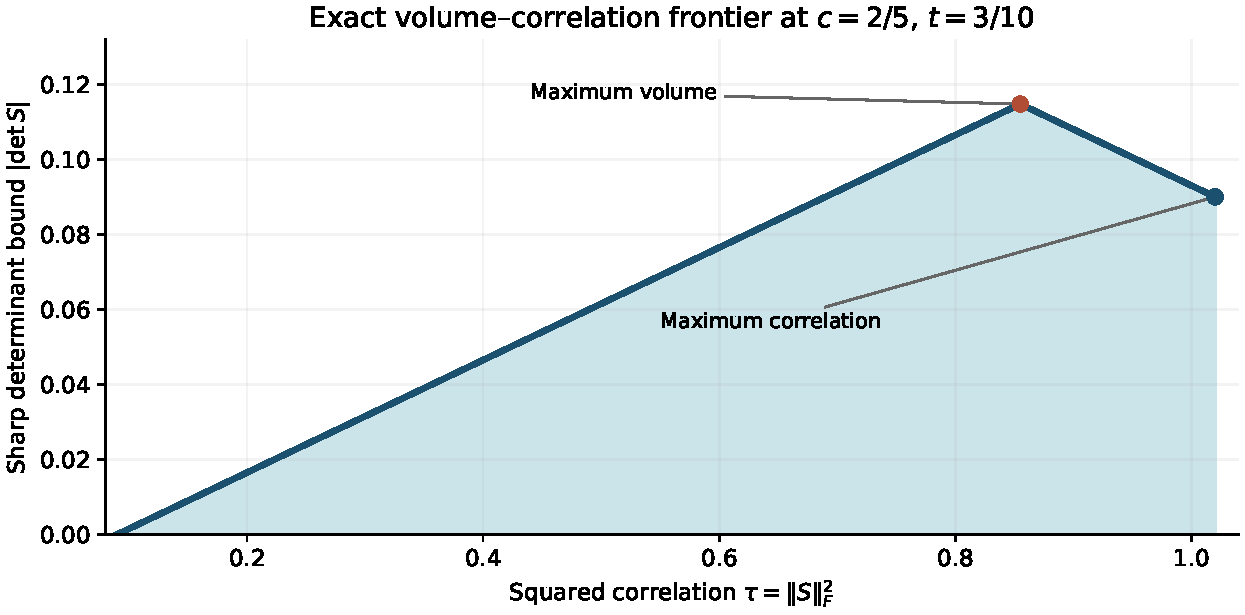
\includegraphics[width=.88\linewidth]{figures/volume_frontier.pdf}
\caption{The exact determinant--correlation frontier at $c=2/5$, $t=3/10$.
The feasible correlation interval is $[0.09,1.02]$. The maximum volume
occurs at $\tau=0.855$, with $|\det S|=0.11475$; at maximum correlation,
$|\det S|=0.09$. Each boundary value has an explicit positive density-matrix
witness, including all singular endpoints.}
\end{figure}

\begin{figure}[htbp]
\centering
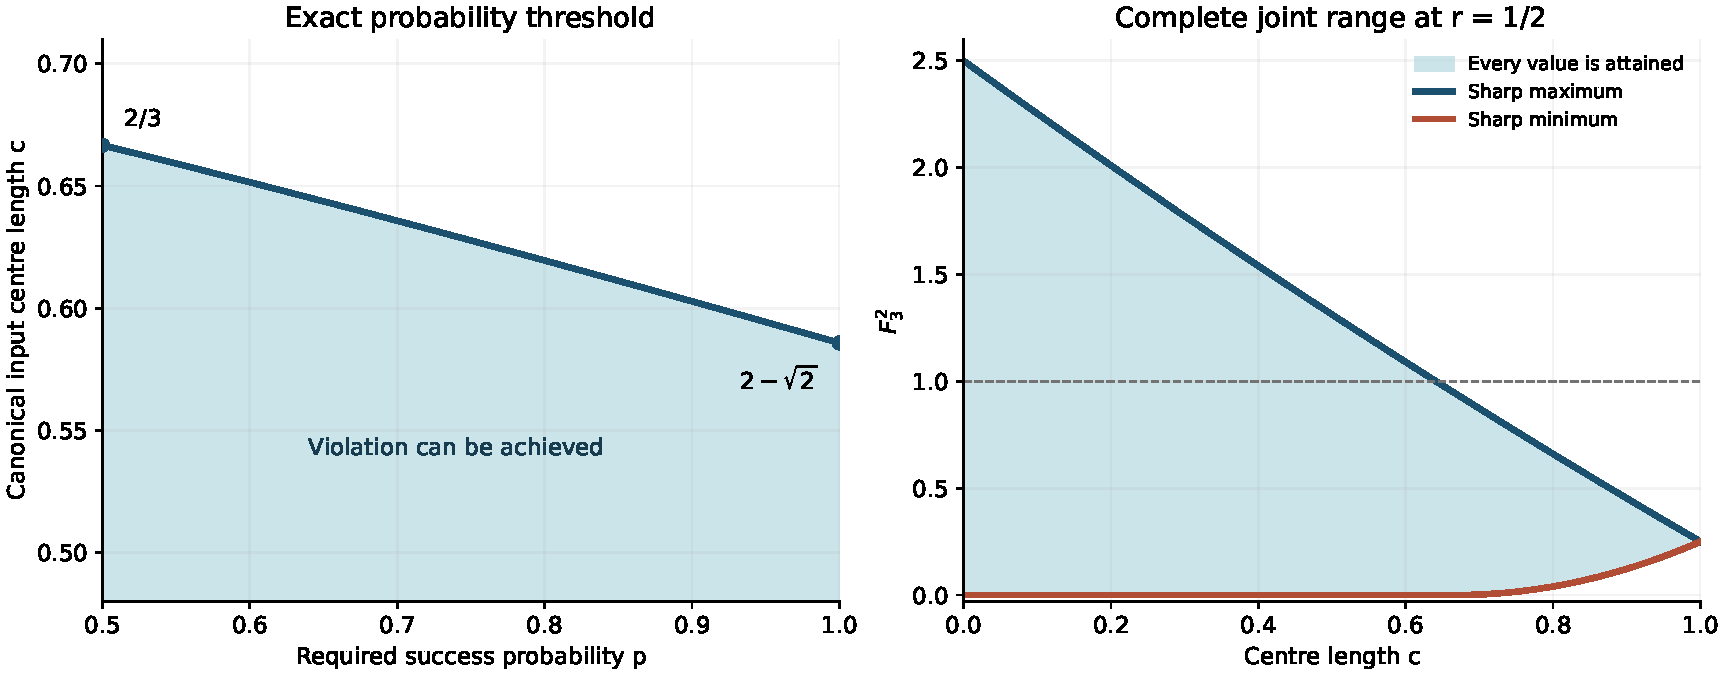
\includegraphics[width=\linewidth]{figures/new_frontiers.pdf}
\caption{Two exact refinements. Left: the strict activation region lies below
$C_{\rm crit}(p)$, optimizing over canonical inputs at each centre. Right: every point between the
sharp lower and upper curves is attained at Bob Bloch length $r=1/2$.
The dashed line is the $F_3^2=1$ threshold.}
\end{figure}

\section{Complete equality classification}\label{sec:classification}
Appendix~\ref{sec:matrix-rigidity} gives the constructive unitary and matrix
proofs behind the formal classification, including repeated eigenvalues,
vanishing coherences, and the pure-product endpoint.
\begin{theorem}[Extremizing states]\label{thm:classification}
For $0<c<2/3$, every state attaining $G(c)$ is locally unitarily equivalent
to \eqref{eq:globalwitness} with $r=r_*(c)$. At $c=0$, the maximizers are
exactly the maximally entangled pure states. There are no maximizers for
$2/3\leq c<1$. At $c=1$, the maximizers are exactly pure product states.
\end{theorem}
\begin{proof}
First classify canonical equality in $\tr Q\leq(1-c)(3-c)$.
Rotate Alice so $\cc=c\mathbf e_z$, and Bob so
$S^{\mathsf T}\mathbf e_z=t\mathbf e_z$, $t\geq0$. At $c=0$, choose any
Alice direction before this rotation. The general canonical matrix now has form
\begin{equation}\label{eq:normal}
\sigma=\begin{pmatrix}
a_+&0&z&w\\0&a_-&v&-z\\
\overline z&\overline v&d_-&0\\\overline w&-\overline z&0&d_+
\end{pmatrix}.
\end{equation}
The diagonal Bob-valued blocks sum to $\Id/2$, commute, and were simultaneously
diagonalized by the Bob rotation. The zero Alice transverse Bloch components
give the $z,-z$ constraint. Direct computation yields
\begin{equation}\label{eq:normalcorr}
\tr Q=t^2+16|z|^2+8|w|^2+8|v|^2.
\end{equation}
Canonical equality and \eqref{eq:radialgap} force $t=1-c$. Then $d_-=0$.
Positivity of $2\times2$ principal minors forces the entire third row and
column to vanish, so $z=v=0$. Equation~\eqref{eq:normalcorr} forces
$|w|=\sqrt{1-c}/2$. A local $Z$ rotation makes $w$ nonnegative, yielding exactly
$\sigma_{c,1-c}$. This argument includes all zero diagonal entries.
At $c=1$, the canonical state is pure on Alice and maximally mixed on Bob.

For $0<c<2/3$, \eqref{eq:square} and the nonnegative losses in
Section~\ref{sec:rigidity} force $r=r_*$, canonical equality, and equality in
\eqref{eq:marginal}. Here $0<r_*<1$, so equality in the triangle inequality
requires the conditional Bloch vector
$\yy=\cc+S\widehat{\bb}$ to equal $\mathbf e_z$.
In the aligned obese form
$S=\operatorname{diag}(\sqrt{1-c},-\sqrt{1-c},1-c)$ this forces
$\widehat{\bb}=\mathbf e_z$. The state is therefore
\eqref{eq:globalwitness} with its unique filter length.
For $c=0$, the square term forces $r=0$ and the canonical equality class is
the Bell orbit. The flat and endpoint cases follow from Theorem~\ref{thm:global}
and the product calculation at $r=1$.
\end{proof}

At fixed $(c,r)$ with $r<1$, the same reasoning classifies equality in
\eqref{eq:joint}. For $0<c<1$, the canonical state must be maximally obese;
when $r>0$ the filter points toward its outward contact with the Bloch sphere.
At $r=0$ there is no filter direction. At $c=0$ equality consists of pure
states with the specified marginal length $r$; at $c=1$ it consists of a
pure Alice state times a Bob state of length $r$. At $r=1$ every state is a
product and $F_3^2=c^2$.

\section{Exact losses and quantitative rigidity}\label{sec:rigidity}
The following is stronger than the original centre-only estimate because it
records separately where each loss occurs.
\begin{proposition}[Exact deficit identity]\label{prop:deficit}
For $0\leq c<2/3$ and $r<1$, put
$\delta=3-4c+c^2-\norm S_F^2$. Then
\begin{equation}\label{eq:deficit}
G(c)-F_3^2=D(c)(r-r_*)^2+(1-r^2)\delta
+[c+(1-c)r]^2-\norm\aa^2.
\end{equation}
All three terms are nonnegative. Thus equality is equivalent to the
simultaneous vanishing of these three explicitly defined matrix losses.
If $c>0$, this implies the sharper geometric inequality
\begin{equation}\label{eq:strongrigidity}
G(c)-F_3^2\geq D(c)(r-r_*)^2
+2(1-r^2)\big((1-c)^2-q\big).
\end{equation}
\end{proposition}
\begin{proof}
Subtract \eqref{eq:filteridentity} from \eqref{eq:square} together with
the definition of $H_c(r)$. Nonnegativity follows from the canonical and
marginal bounds. Then apply \eqref{eq:radialgap}.
\end{proof}

There is a more detailed identity. For $0<c<2/3$ and $0<r<1$, set
$\nn=\cc/c$, $\yy=\cc+S\widehat{\bb}$, and
$\tau=4\Tr(\sigma\sigma_{\nn})=1-c^2+2q-\tr Q$. Then
\begin{align}\label{eq:five}
G(c)-F_3^2={}&D(c)(r-r_*)^2+(1-r^2)\{2[(1-c)^2-q]+\tau\}\nonumber\\
&+r[r+c(1-r)](1-\norm\yy^2)+rc(1-r)\norm{\yy-\nn}^2.
\end{align}
Each displayed contribution is nonnegative. The last line follows by
expanding $\aa=(1-r)c\nn+r\yy$ and using
$2(1-\nn\cdot\yy)=1-\norm\yy^2+\norm{\yy-\nn}^2$.
At $r=0$ the endpoint terms vanish; at $c=0$ use \eqref{eq:deficit} without
dividing by $c$. The five losses correspond to filter length, radial support
width, spin-flip overlap, conditional-state impurity, and endpoint direction.

\begin{theorem}[Explicit stability of the canonical optimizer]\label{thm:stability}
For a canonical state with $0\leq c<1$, put $d=1-c$, let $t$ be the radial
support half-width, and put $\delta=3-4c+c^2-\tr Q$.
There exist local unitaries $U_A,U_B$ such that, with $U=U_A\otimes U_B$,
\begin{align}\label{eq:stability}
\norm{U\sigma U^\dagger-\sigma_{c,d}}_1^2
&\leq\min\left\{4,\left[\frac12+\frac{2+c}{d+t}\right]\delta\right\}\nonumber\\
&\leq\min\left\{4,\frac{5+c}{2(1-c)}\delta\right\}.
\end{align}
The norm is the trace norm. For the convention that trace distance is one
half of that norm, divide the square-root bounds by two. The constants are
proved upper bounds and are not claimed optimal.
\end{theorem}
\begin{proof}
Use \eqref{eq:normal}; make $w\geq0$ by a local phase rotation. Let
$y=d-t\in[0,d]$ and $w_0=\sqrt d/2$. Principal-minor positivity gives
\[
w^2\leq a_+d_+\leq w_0^2,\qquad |z|^2\leq a_+y/4,\qquad
|v|^2\leq a_-y/4.
\]
In particular,
\begin{equation}\label{eq:minorbound}
16(2|z|^2+|v|^2)\leq y(3+3c+t)=y(4+2c-y).
\end{equation}
Equation~\eqref{eq:normalcorr} implies exactly
\[
\delta=(d^2-t^2)+8(w_0^2-w^2)-16|z|^2-8|v|^2.
\]
Since $0\leq w\leq w_0$, $(w_0-w)^2\leq w_0^2-w^2$.
The four diagonal differences from $\sigma_{c,d}$ are $\pm y/4$, so
\[
\norm{\sigma-\sigma_{c,d}}_F^2=y^2/4+4|z|^2+2|v|^2+2(w_0-w)^2.
\]
For $4\times4$ matrices, Cauchy--Schwarz on singular values gives
$\norm X_1^2\leq4\norm X_F^2$. Retaining the radial deficit term yields
\begin{align*}
\norm{\sigma-\sigma_{c,d}}_1^2
&\leq\delta+y^2-(d^2-t^2)+16(2|z|^2+|v|^2)\\
&\leq\delta+y(3+3c-t).
\end{align*}
By \eqref{eq:radialgap}, $\delta\geq2y(d+t)$. Since $d+t>0$ and
$3+3c-t\geq0$, we obtain
\[
\norm{\sigma-\sigma_{c,d}}_1^2\leq
\delta\left[1+\frac{3+3c-t}{2(d+t)}\right]
=\delta\left[\frac12+\frac{2+c}{d+t}\right].
\]
Use $d+t\geq d$ for the uniform version and
$\norm{\sigma-\sigma_{c,d}}_1\leq2$ for the other branch. None of the
arguments divides by a diagonal entry or assumes a full-rank state.
\end{proof}

In particular, if $F_3(\rho)^2\geq G(c)-\varepsilon$, $c<2/3$, and $r<1$, then
\[
|r-r_*|\leq\sqrt{\varepsilon/D(c)},\qquad
\delta\leq\frac{\varepsilon}{1-r^2}.
\]
The whitened state is therefore, up to local unitaries, within trace norm
\[
\min\left\{2,\sqrt{\frac{(5+c)\varepsilon}{2(1-c)(1-r^2)}}\right\}
\]
of the canonical obese optimizer. This conclusion concerns the whitened
state; it is not a claimed trace-distance bound to the globally optimal
\emph{unfiltered} state.

\subsection{Extremizing sequences and a sharp change in stability exponent}
The unattained branch has a different stability phenomenon from the curved
branch. Its limiting pure products have centre length one, even when every
state in the sequence has the same smaller centre length.

\begin{theorem}[Sharp rates on the unattained branch]\label{thm:flatstability}
Fix $2/3\leq c<1$. If a sequence of states with centre length $c$ has
$F_3(\rho_j)^2\to1$, then eventually its Bob marginals are full rank,
$r_j\to1$, and its distance to the set $\mathcal P$ of pure product states
tends to zero. Put
\[
\varepsilon=1-F_3(\rho)^2,\quad h=1-r,\quad
A=4c-2-c^2,\quad B=6c-4,\quad D=2-2c-c^2.
\]
For $r<1$,
\begin{equation}\label{eq:flatrate}
\varepsilon\geq Ah^2+B(1-h)h=Bh+Dh^2,\qquad
\inf_{\pi\in\mathcal P}\norm{\rho-\pi}_1^2\leq2\varepsilon+14h.
\end{equation}
Consequently, at fixed $c$, as $\varepsilon\downarrow0$,
\begin{equation}\label{eq:criticalrate}
\inf_{\pi\in\mathcal P}\norm{\rho-\pi}_1=
\begin{cases}
O(\varepsilon^{1/4}),&c=2/3,\\
O(\varepsilon^{1/2}),&2/3<c<1.
\end{cases}
\end{equation}
Both exponents are sharp: neither can be increased in a bound valid for all
states at the specified fixed centre length.
\end{theorem}
\begin{proof}
A state with $r=1$ has $F_3^2=c^2<1$, so such states cannot occur arbitrarily
late in an extremizing sequence. Equation~\eqref{eq:flat} gives the first
bound in \eqref{eq:flatrate}. Since $A>0$ and $B\geq0$, it forces $h\to0$.
The exact filter identity gives
\[
1-\norm\aa^2=\varepsilon+(1-r^2)(\norm S_F^2-c^2)
\leq\varepsilon+3(1-r^2)\leq\varepsilon+6h.
\]
Choose the top eigenvectors of both marginal states and let $\pi$ be their
product projector. The elementary union bound for their commuting projectors
gives $\Tr(\rho\pi)\geq(\norm\aa+r)/2$. The pure-target trace-norm bound
$\norm{\rho-\pi}_1\leq2\sqrt{1-\Tr(\rho\pi)}$ follows, for example, by
spectral decomposition, the pure-state formula, and concavity of the square
root. Since $1-\norm\aa\leq1-\norm\aa^2$, this proves
the second inequality in \eqref{eq:flatrate}.

At $c=2/3$, $B=0$ and $D=2/9$, so
$h\leq3\sqrt{\varepsilon}/\sqrt2$. At fixed $c>2/3$, once $h\leq1/2$,
the first expression in \eqref{eq:flatrate} gives
$h\leq2\varepsilon/B$. Substitution proves \eqref{eq:criticalrate}.

For sharpness, take $\rho_{c,1-h}$ from \eqref{eq:globalwitness}.
It has exactly $\varepsilon=Bh+Dh^2$. Let
$W=(|\psi^-\rangle\langle\psi^-|)^{\Gamma_B}$, with
$|\psi^-\rangle=(|01\rangle-|10\rangle)/\sqrt2$.
This operator has operator norm $1/2$ and nonnegative expectation in every separable
state, because its expectation in a product is a squared overlap with a
partially conjugated product vector. Direct calculation gives
\[
\Tr(W\rho_{c,1-h})=\frac{ch}{4}
-\frac12\sqrt{(1-c)(2h-h^2)}.
\]
Trace-norm duality therefore implies, even for the distance to the larger
set of separable states,
\begin{equation}\label{eq:flatlower}
\inf_{\pi\in\mathcal P}\norm{\rho_{c,1-h}-\pi}_1
\geq\sqrt{(1-c)(2h-h^2)}-\frac{ch}{2}.
\end{equation}
Its leading term is $\sqrt{2(1-c)h}$. At $c=2/3$ the leading lower bound is
$2^{1/4}\varepsilon^{1/4}$; at fixed $2/3<c<1$ it is
$\sqrt{2(1-c)/(6c-4)}\sqrt\varepsilon$. This proves sharpness of both
exponents. The constants are not asserted uniform in $c$, and the case
$c=1$ is the separately attained endpoint.
\end{proof}

For a \emph{fixed} canonical state with $2/3\leq c<1$, the supremum over
invertible Bob filters equals one exactly when its ellipsoid has a pure
contact: $\norm{\cc+S\mathbf u}=1$ for some unit $\mathbf u$.
Indeed, the continuous objective on the closed filter ball has no interior
point of value one, and on the sphere it is exactly
$\norm{\cc+S\mathbf u}^2$. Compactness proves necessity; approaching a pure
contact radially proves sufficiency. For any sequence in this fixed orbit
with $F_3^2\to1$, every cluster point of its filter directions lies in this
contact set. Thus an individual ellipsoid can
have an orbit supremum strictly below the global value one.


\section{An exact test for one-sided hidden \texorpdfstring{$F_3$}{F3} violation}\label{sec:orbit}
The centre bound is a universal obstruction. Using the entire ellipsoid gives
a necessary and sufficient test for whether any Bob-only filter can reveal
$F_3>1$. This directly addresses the asymmetric filtering problem raised
in Eqs.~(9)--(10) and the conclusion of the 2024 paper~\cite{ducuara}.

Fix canonical Bloch data $(\cc,0,S)$ and put
\begin{equation}\label{eq:orbitdefs}
\tau=\norm S_F^2,\qquad \mathbf k=S^{\mathsf T}\cc,\qquad
K=(\tau-c^2)\Id-S^{\mathsf T}S.
\end{equation}
Every positive invertible Bob filter, after normalization, is represented by
$F=\sqrt{\Id+\bb\cdot\bs}$, $\norm\bb<1$. Polar decomposition shows that
post-filter unitaries do not enlarge the achievable $F_3$ values. From
\eqref{eq:filteridentity} and $\aa=\cc+S\bb$, the exact squared value is
\begin{equation}\label{eq:orbitquadratic}
f(\bb)=\tau+2\mathbf k\cdot\bb-\bb^{\mathsf T}K\bb.
\end{equation}
On the unit sphere its continuous boundary value is
\begin{equation}\label{eq:orbitboundary}
f(\bb)=\norm{\cc+S\bb}^2\leq1.
\end{equation}
Boundary parameters represent singular filters producing product states.

\begin{theorem}[One-sided violation criterion and exact optimum]\label{thm:orbit}
Some invertible Bob filter produces $F_3>1$ if and only if
\begin{equation}\label{eq:orbitcriterion}
K\succ0,\qquad \norm{K^{-1}\mathbf k}^2<1,\qquad
V:=\tau+\mathbf k^{\mathsf T}K^{-1}\mathbf k>1.
\end{equation}
When these conditions hold, the maximum squared value is $V$, attained at
the unique positive-filter parameter $\bb_*=K^{-1}\mathbf k$.
Singular or indefinite $K$ cannot permit an $F_3$ violation.
\end{theorem}
\begin{proof}
A value greater than one in the open ball gives, by continuity, a maximum
greater than one on the compact closed ball. Equation~\eqref{eq:orbitboundary}
forces it to be interior. First and second derivative conditions give
$K\bb_*=\mathbf k$ and $K\succeq0$.
If $K$ had a nonzero null vector $\mathbf v$, then
$\mathbf k\cdot\mathbf v=\bb_*^{\mathsf T}K\mathbf v=0$.
The value of $f$ would be constant on the line $\bb_*+s\mathbf v$, which
meets the unit sphere, contradicting \eqref{eq:orbitboundary}.
Thus $K\succ0$. Completing the square gives
\[
f(\bb)=V-(\bb-\bb_*)^{\mathsf T}K(\bb-\bb_*).
\]
This proves the necessary conditions, value, and uniqueness. Conversely,
\eqref{eq:orbitcriterion} places this stationary point in the physical
open ball with value greater than one; the same identity proves optimality.
\end{proof}

For an original state with full-rank Bob marginal, whitening followed by this
filter is one Bob filter, scaled to a valid Kraus contraction. Conversely
every Bob filter is represented in this canonical orbit up to a Bob unitary.
A pure Bob marginal is a product case and never violates. Thus both
possible marginal ranks and every global rank are covered.

\subsection{Ellipsoid-only and exact polynomial forms}
Put $L=(\tau-c^2)\Id-Q$, where $Q=SS^{\mathsf T}$. The matrices $K,L$ have
the same eigenvalues, including when $S$ is singular. Intertwining yields
\begin{equation}\label{eq:geometriccriterion}
L\succ0,\qquad \cc^{\mathsf T}QL^{-2}\cc<1,\qquad
\tau+\cc^{\mathsf T}QL^{-1}\cc>1.
\end{equation}
This equivalent test depends only on the centre and ellipsoid matrix.
For rational data, let $\ell=\det L$ and $R=\operatorname{adj}L$.
After certifying $L\succ0$ by principal minors, so $\ell>0$, the other tests are
\[
\cc^{\mathsf T}QR^2\cc<\ell^2,\qquad
(\tau-1)\ell+\cc^{\mathsf T}QR\cc>0.
\]
These are finite polynomial inequalities and require no numerical inverse.

The unit-ball condition cannot be dropped. The positive definite canonical state
\[
\sigma=\frac1{40}\begin{pmatrix}19&0&0&5\\0&7&1&0\\0&1&1&0\\5&0&0&13\end{pmatrix}
\]
has two positive $2\times2$ blocks with determinants $222/1600$ and $6/1600$.
Its data are $\cc=(0,0,3/10)$, $S=\operatorname{diag}(3/10,-1/5,3/5)$,
$\tau=49/100$, $K=\operatorname{diag}(31,36,4)/100\succ0$.
The unconstrained vertex is $(0,0,9/2)$ with value $13/10>1$, outside the
physical ball. The actual supremum is $81/100<1$, from
\[
f(x,y,z)=\frac{49}{100}+\frac9{25}z-\frac{31}{100}x^2
-\frac9{25}y^2-\frac1{25}z^2.
\]
It increases with $z$ on $[-1,1]$, and its transverse terms are nonpositive.

The criterion gives another proof of the threshold. For $c>0$ and
$q=\nn^{\mathsf T}Q\nn$, $\nn=\cc/c$, some direction perpendicular to $\nn$
has Rayleigh quotient at least $(\tau-q)/2$. Hence
\[
\lambda_{\min}(L)\leq\frac{\tau+q-2c^2}{2}
\leq\frac{1-3c^2+3q}{2}\leq2-3c.
\]
For $c\geq2/3$, the necessary positive-definiteness condition fails.

\subsection{The entire orbit supremum, including singular quadratic cases}
For completeness, the exact scalar trust-region characterization is
\begin{equation}\label{eq:trustregion}
\sup_{\norm\bb<1}f(\bb)=\tau+
\min_{\substack{\lambda\geq0,\ K+\lambda\Id\succeq0\\
\mathbf k\in\operatorname{range}(K+\lambda\Id)}}
\left[\lambda+\mathbf k^{\mathsf T}(K+\lambda\Id)^\dagger\mathbf k\right].
\end{equation}
Here $\dagger$ is the Moore--Penrose inverse. For the upper bound, put
$B=K+\lambda\Id$ and complete the square:
\[
f(\bb)=\tau+\lambda\norm\bb^2+\mathbf k^{\mathsf T}B^\dagger\mathbf k
-(\bb-B^\dagger\mathbf k)^{\mathsf T}B(\bb-B^\dagger\mathbf k).
\]
For equality, use $\lambda=0$ if $K\succeq0$,
$\mathbf k\in\operatorname{range}K$, and $\norm{K^\dagger\mathbf k}\leq1$.
Otherwise let $\lambda_0=\max(0,-\lambda_{\min}(K))$. For
$\lambda>\lambda_0$, $\norm{(K+\lambda\Id)^{-1}\mathbf k}$ is continuous,
nonincreasing, and tends to zero. If its limit at $\lambda_0$ exceeds one,
choose a root with norm one. If the limit is at most one, the excluded
$\lambda=0$ case implies $\lambda_0>0$; the limiting matrix is singular
and $\mathbf k$ is orthogonal to its kernel. Add a kernel vector to its
minimum-norm solution to reach the unit sphere. The square term vanishes in
both cases, giving equality. The open ball has the same supremum as its
closure by continuity, but need not attain a boundary optimum.

In a $K$ eigenbasis, the scalar objective is
$\lambda+\sum_i k_i^2/(\kappa_i+\lambda)$; a zero denominator is admissible
only when the corresponding numerator vanishes. Unlike the formula in the
violating regime, this exact characterization retains a scalar minimization.


\section{Complete one-sided orbit optimization, including all hard cases}
\label{sec:complete-trust-region}

The generic optimization method in this section is classical trust-region
theory; see Mor\'e--Sorensen (1983) and Fortin--Wolkowicz (2004).  The extension
here is its exact application to the complete physical one-sided $F_3$ orbit,
with singular filters retained, together with a constructive formal proof.
In particular, a scalar minimization is not left as the answer: an explicitly
tested spectral endpoint or one uniquely admissible root of a degree-six
polynomial determines the result.

\subsection{Spectral algorithm for an arbitrary real quadratic}

Let $K=K^T\in\mathbb R^{3\times3}$, $k\in\mathbb R^3$, and $\tau\in\mathbb R$.
We seek the exact maximum of
\begin{equation}
 f(x)=\tau+2k^Tx-x^TKx,\qquad \|x\|\leq1.
 \label{eq:full-orbit-quadratic}
\end{equation}
Choose an orthogonal diagonalization
\[
 K=U\operatorname{diag}(d_1,d_2,d_3)U^T,\qquad h=U^Tk,
 \qquad d_{\min}=\min_i d_i,
 \qquad L=\max\{0,-d_{\min}\}.
\]
For $\ell\geq L$, define the partial reciprocal vector and its squared norm by
\[
 q_i(\ell)=
 \begin{cases}h_i/(d_i+\ell),&d_i+\ell\ne0,\\0,&d_i+\ell=0,\end{cases}
 \qquad \psi(\ell)=\sum_i q_i(\ell)^2.
\]
The zero-denominator convention alone does not make the endpoint admissible:
the range condition below must also hold.

\paragraph{Exact finite algorithm.}
First test the endpoint condition
\begin{equation}
 h_i=0\quad\hbox{whenever }d_i+L=0,
 \qquad \psi(L)\leq1.
 \label{eq:floor-admissibility}
\end{equation}
If it holds, set $\ell_*=L$.  If it fails, let $\ell_*>L$ be the unique solution of
\begin{equation}
 \sum_{i=1}^3\frac{h_i^2}{(d_i+\ell_*)^2}=1.
 \label{eq:regular-secular}
\end{equation}
This regular equation is equivalently the polynomial equation
\begin{align}
 P(\ell)={}&h_1^2(d_2+\ell)^2(d_3+\ell)^2
 +h_2^2(d_1+\ell)^2(d_3+\ell)^2\notag\\
 &+h_3^2(d_1+\ell)^2(d_2+\ell)^2
 -(d_1+\ell)^2(d_2+\ell)^2(d_3+\ell)^2=0.
 \label{eq:secular-polynomial}
\end{align}
Its degree is exactly six, with leading coefficient $-1$, including when
$h=0$ or eigenvalues coincide.  Consequently the endpoint and the real roots
of $P$ form a set of at most seven candidates.  The endpoint test
\eqref{eq:floor-admissibility} and the regular restriction $\ell>L$ select
exactly one admissible candidate.  Clearing denominators introduces no
spurious candidate on that regular interval, because every denominator is
strictly positive there.  In the original coordinates the same regular
polynomial equation can be written
\[
 \|\operatorname{adj}(K+\ell I)k\|^2-\det(K+\ell I)^2=0.
\]
The spectral version is particularly convenient for explicitly resolving the
singular endpoint.

\paragraph{Exact maximum and every maximizing point.}
The answer is
\begin{equation}
 M=\tau+\ell_*+
 \sum_{i:\,d_i+\ell_*\ne0}\frac{h_i^2}{d_i+\ell_*}.
 \label{eq:complete-orbit-value}
\end{equation}
Put $q=q(\ell_*)$ and
$E_* = \{z\in\mathbb R^3:z_i=0\text{ whenever }d_i+\ell_*\ne0\}$.
The complete maximizing set is
\begin{equation}
 \left\{U(q+z):z\in E_*,\quad
 \begin{cases}
  \|z\|^2\leq1-\psi(\ell_*),&\ell_*=0,\\
  \|z\|^2=1-\psi(\ell_*),&\ell_*>0.
 \end{cases}\right\}.
 \label{eq:complete-orbit-maximizers}
\end{equation}
The endpoint range condition guarantees $h_i=0$ on $E_*$, and $q$ is
orthogonal to $E_*$.  Thus this description includes every degenerate case:

\begin{itemize}
\item If $\ell_*>L$, all shifted eigenvalues are positive, and the unique
maximizer is $Uq$, on the unit sphere.
\item If $\ell_*=0$, the original $K$ is positive semidefinite.  The
maximizers form the explicitly displayed affine ball in $\ker K$.
For $K\succ0$ this is the single unconstrained vertex $K^{-1}k$.
\item If $\ell_*=L>0$, then $d_{\min}<0$ and $h$ is orthogonal to the
lowest-eigenvalue eigenspace.  This is the hard case.  The missing radius
is supplied by a vector in that eigenspace, giving precisely the sphere
in \eqref{eq:complete-orbit-maximizers}.  When its radius is zero the
maximizer is nevertheless unique.
\item If $k=0$, the formula reduces to $M=\tau+\max\{0,-d_{\min}\}$.
For $d_{\min}>0$ the maximizer is zero; for $d_{\min}=0$ it is the unit
ball in the kernel; for $d_{\min}<0$ it is the unit sphere in the
lowest-eigenvalue eigenspace.  This includes $K=0$.
\end{itemize}

\subsection{Constructive proof, without assumed optimality conditions}

In the eigenbasis, write $y=U^Tx$ and
$f_D(y)=\tau+\sum_i(2h_i y_i-d_i y_i^2)$.
We construct $p$ and $\ell$ satisfying
\begin{equation}
 \ell\geq0,\quad d_i+\ell\geq0,\quad
 (d_i+\ell)p_i=h_i,\quad
 \|p\|\leq1,\quad \ell(1-\|p\|^2)=0.
 \label{eq:constructed-certificate}
\end{equation}
These conditions are conclusions of the construction, not hypotheses
substituted for the optimization problem.

Suppose first that \eqref{eq:floor-admissibility} holds.
At $\ell=L=0$, take $p=q(L)$.  At $\ell=L>0$, choose an index $j$ for
which $d_j+L=0$, and set
\[
 p=q(L)+\sqrt{1-\psi(L)}\,e_j.
\]
The range condition gives $q_j(L)=h_j=0$, so $\|p\|=1$ and every equation
in \eqref{eq:constructed-certificate} holds.  This directly treats the
hard case, including repeated lowest eigenvalues and a zero linear term.

If the endpoint is inadmissible, a regular root exists by a finite bracket.
When the range condition holds but $\psi(L)>1$, choose $a=L$.
If instead $d_j+L=0$ and $h_j\ne0$ for some $j$, choose
$a=L+|h_j|/2$.  The $j$th summand of $\psi(a)$ is then exactly $4$,
so $\psi(a)>1$.  In either case all denominators at $a$ are nonnegative,
and any zero denominator has zero numerator.  The function $\psi$ is
therefore continuous on $[a,\infty)$.  For the explicit endpoint
\[
 b=a+1+\|h\|
\]
we have
\[
 \psi(b)\leq\frac{\|h\|^2}{(1+\|h\|)^2}<1.
\]
The intermediate value theorem gives a root $\ell\in(a,b)$, hence
$\ell>L$.  Now take $p=q(\ell)$; this proves
\eqref{eq:constructed-certificate} in the remaining case.  No compactness
or differentiability assumption about an unknown optimizer was needed.

For every such constructed certificate and every $y\in\mathbb R^3$,
direct expansion yields the exact gap identity
\begin{equation}
 f_D(p)-f_D(y)=
 \sum_i(d_i+\ell)(y_i-p_i)^2+\ell(1-\|y\|^2).
 \label{eq:trust-exact-gap}
\end{equation}
Both terms are nonnegative on the ball, proving global optimality.
Equality holds exactly when $y_i=p_i$ for every strictly positive
$d_i+\ell$, together with $\ell(1-\|y\|^2)=0$.
This proves \eqref{eq:complete-orbit-maximizers}.  Multiplying each
stationary equation by $p_i$ and using complementarity gives
\eqref{eq:complete-orbit-value}.

For completeness, the admissible shift is also unique in the hard and flat
cases.  Let $(p,\ell)$ and $(q,m)$ be two certificates.  Each point is
globally maximizing, so equality in \eqref{eq:trust-exact-gap} gives
$(d_i+\ell)q_i=h_i$ and $\ell(1-\|q\|^2)=0$.
Subtracting $(d_i+m)q_i=h_i$ yields $(m-\ell)q_i=0$ for every $i$.
If $m\ne\ell$, then $q=0$, and the two complementarity equations force
$m=\ell=0$, a contradiction.  Thus the algorithm selects one shift even
when it selects a continuum of maximizing vectors.

Equivalently, in the original coordinates, a point $x$ is globally
maximizing if and only if it belongs to the unit ball and there exists
$\ell\geq0$ with
\[
 K+\ell I\succeq0,\qquad (K+\ell I)x=k,
 \qquad \ell(1-\|x\|^2)=0.
\]
The proof above establishes existence of this global certificate for every
real symmetric $K$, rather than assuming this characterization.

\subsection{Exact application to all canonical quantum-filter orbits}

Let $\sigma$ be any actual two-qubit density matrix with Bob marginal $I/2$,
Alice Bloch vector $c\in\mathbb R^3$, and correlation matrix $S$.
Set
\begin{equation}
 \tau=\|S\|_F^2,\qquad k=S^Tc,\qquad
 K=(\tau-\|c\|^2)I-S^TS.
 \label{eq:physical-trust-data}
\end{equation}
For every complex $2\times2$ filter $F$ normalized by
$\operatorname{Tr}(F^\dagger F)=2$, there is an $x$ in the closed unit ball
such that $F^\dagger F=I+x\cdot\sigma$.  The actual normalized output
$\rho_F=(I\otimes F)\sigma(I\otimes F^\dagger)$ satisfies the exact identity
\begin{equation}
 F_3(\rho_F)^2=\tau+2k^Tx-x^TKx.
 \label{eq:physical-complete-objective}
\end{equation}
Conversely every such $x$ is realized by the positive filter
$F=(I+x\cdot\sigma)^{1/2}$.  These statements hold at every joint-state
rank and include singular filters.

Apply the finite algorithm to \eqref{eq:physical-trust-data}.
The exact maximum over all normalized complex one-sided filters is the
number $M$ in \eqref{eq:complete-orbit-value}, and the exact maximum of
$F_3$ is $\sqrt M$.  Every maximizing effect, and no other effect, is
\[
 F^\dagger F=I+\bigl(U(q+z)\bigr)\cdot\sigma,
\]
with $z$ exactly as in \eqref{eq:complete-orbit-maximizers}.  All complex
filters with a given maximizing effect are included; no Hermiticity
restriction is imposed on $F$.  A positive square-root filter explicitly
realizes each maximizing effect.

This completes the orbit optimization even when its maximum is at or below
the steering threshold.  The earlier violation criterion is recovered as
the special case in which the physical sphere bound $F_3^2\leq1$ forces
an interior optimizer with $K\succ0$.

\subsection{Invertible filters: supremum versus attainment}

For normalized filters,
\[
 \det(F^\dagger F)=1-\|x\|^2,
\]
so invertibility is equivalent to $\|x\|<1$.  The exact supremum over
invertible filters is still $M$: if $x_*$ is any closed-ball maximizer,
the effects $t x_*$ with $0\leq t<1$ are realized by invertible positive
filters, and their values tend to $M$ as $t\uparrow1$.

An invertible filter attains that supremum if and only if
\begin{equation}
 \ell_*=0\quad\hbox{and}\quad\psi(\ell_*)<1.
 \label{eq:invertible-attainment}
\end{equation}
Indeed positive shift forces every optimizer onto the unit sphere.
At zero shift the squared norm of $q+z$ is
$\psi(0)+\|z\|^2$, and an interior point exists exactly under
\eqref{eq:invertible-attainment}.  In particular, an endpoint maximum
can be attained by singular filters while only being approached by
invertible ones.  This distinction is not removed by assuming that the
input joint state has full rank.

\subsection{State rank, quadratic rank, and filter rank are different}
Two full-rank physical examples show why the singular cases cannot be
removed by imposing positivity on the input state.

First take
\[
 \sigma=\frac{I+cZ}{2}\otimes\frac I2,\qquad 0<c<1.
\]
Here $S=0$, $k=0$, and $K=-c^2I$. The objective is
$f(x)=c^2\|x\|^2$. Its maximum is $c^2$, every unit vector maximizes,
and the spectral shift is $\ell_*=c^2$. This is a hard case with a
three-dimensional nullspace of $K+\ell_*I$. Every maximizing filter is
singular, and the same value is only a supremum for invertible filters,
even though the input density matrix has rank four.

Next take
\[
 \sigma=\frac14(I+tX\otimes X),\qquad 0<t<1.
\]
This state also has rank four, but now $k=0$ and
$K=\operatorname{diag}(0,t^2,t^2)$. The exact maximum is $t^2$ and every
point $x=(s,0,0)$ with $|s|\leq1$ is a maximizer. Thus the complete
maximizing effect set contains both invertible and singular filters.
These are direct specializations of the universal checked theorem.
The exact rational certificate file includes both types of example.

\paragraph{Verification scope.}
The accompanying formal-coverage manifest identifies the exact Lean
declarations and compiler evidence for the results above.  Numerical
comparisons are reproducibility checks only; no numerical result is a
logical premise of a formal theorem.


\section{Scope}\label{sec:scope}
The results concern the matrix quantity $F_3=\norm T_{\mathrm F}$ in the
convention of Eq.~(3) of~\cite{ducuara}; $F_3\leq1$ does not prove the
existence of a local hidden-state model for all measurements. If Bob's
measurement triad is fixed and only Alice's directions are optimized, the
value can be smaller. The success probabilities refer to canonical inputs;
an arbitrary original input has a separate whitening cost. The actual
centre of a singularly filtered output is handled separately from the
input centre. The explicit trace-norm stability constants are upper bounds
and are not claimed to be optimal.

\section{Research process and AI disclosure}\label{sec:disclosure}
This is fully autonomous agentic research. The results, their proofs, the
Lean development, the exact and numerical checkers and a draft report were
produced by autonomous AI research agents, which took the earlier
package~\cite{earlier} as their starting point; their records describe
internal reviews carried out within the same automated workflow and do not
name the system used.

Opus~5.5 by Anthropic used with Claude Code assessed the work for this
release. It read the proofs of the joint interval, the canonical interval,
the probability frontier and the volume bounds, compared the principal
Lean statements with the mathematics, reran every checker from a copy,
wrote the exact check \path{calculations/independent/exact_new_results.py},
added the whole-project axiom audit, ran the fresh Lean build recorded in
\path{verification/}, and edited this manuscript from the draft report.
The remaining proofs were carried over and read, but not all were
rederived line by line.

Dev D. Goyal is responsible for publication. The work has not been
externally peer reviewed; AI checks are not human peer review, no expert
validation is claimed, and the literature comparison is bounded and does
not establish priority. Appendix~\ref{sec:verification} states the formal
scope and its limits.

\appendix
\section{Constructive matrix proofs of rigidity and extremizer classification}
\label{sec:matrix-rigidity}

The equality and stability results in this section concern actual complex
density matrices and actual qubit unitaries.  In particular, no unproved
rotation-to-unitary lifting assertion is used.  Write
\(\tau(\sigma)=\|T(\sigma)\|_F^2\), and use the trace norm
\(\|X\|_1=\sum_j|\lambda_j(X)|\) for Hermitian \(X\).
The usual trace distance between states is \(\frac12\|\rho-\sigma\|_1\).

\subsection{A complete radial normal form, including degenerate cases}

For a canonical state, Bob's marginal is \(I/2\).  First diagonalize Alice's
marginal by a qubit unitary, putting her Bloch vector at \(c e_z\), where
\(c\geq0\).  In Alice blocks write
\(\sigma=\left(\begin{smallmatrix}A&C\\C^\dagger&D\end{smallmatrix}\right)\).
Then \(A+D=I/2\).  A second qubit unitary, acting only on Bob, diagonalizes
the Hermitian matrix \(H=A-D\), with its eigenvalues in decreasing order.
If their difference is \(t\geq0\), the resulting state is exactly
\begin{equation}
 M(c,t,z,w,v)=
 \begin{pmatrix}
 a_+&0&z&w\\
 0&a_-&v&-z\\
 \overline z&\overline v&d_-&0\\
 \overline w&-\overline z&0&d_+
 \end{pmatrix},\qquad
 a_\pm=\frac{1+c\pm t}{4},\quad
 d_\pm=\frac{1-c\pm t}{4}.
 \label{eq:rigidity-normal-form}
\end{equation}
Positivity implies \(0\leq t\leq1-c\).  Both spectral diagonalizations
remain valid for repeated eigenvalues and singular density matrices.
The trace-zero condition on \(C\), which forces its diagonal entries to
be \(z,-z\), follows from the vanishing off-diagonal entry of Alice's
marginal.

There is also a version with a prescribed radial axis.  If Alice's Bloch
vector is already \(c e_z\), diagonalize only \(H=A-D\).  Direct Pauli
expansion gives
\begin{equation}
 \operatorname{BlochSq}(H)=\|T^{\mathsf T}e_z\|^2=t^2.
\end{equation}
Thus the prescribed \(t\) is preserved.  This statement holds even when
\(c=0\): the marked axis is still \(e_z\), and Alice's unitary is exactly
the identity.  Diagonalizing a maximally mixed Alice marginal alone would
not justify preservation of an arbitrary marked axis.

In the normal form,
\begin{equation}
 \tau=t^2+16|z|^2+8|w|^2+8|v|^2.
 \label{eq:normal-form-correlation}
\end{equation}
The sharp geometric inequality \(\tau\leq1-c^2+2t^2\) has the following
complete equality conditions:
\begin{align}
 t z&=0,\label{eq:rigidity-equality-one}\\
 |z|^2+|w|^2&=a_+d_+,\label{eq:rigidity-equality-two}\\
 |z|^2+|v|^2&=a_-d_-,\label{eq:rigidity-equality-three}\\
 z\overline v&=w\overline z.\label{eq:rigidity-equality-four}
\end{align}
These are necessary and sufficient for every positive matrix
\eqref{eq:rigidity-normal-form}.  For \(t>0\), they reduce to
\begin{equation}
 z=0,\qquad |w|^2=a_+d_+,\qquad |v|^2=a_-d_-.
 \label{eq:positive-t-equality}
\end{equation}
Thus all extremizers in this basis are the explicit two-block states
\eqref{eq:positive-t-equality}, including arbitrary admissible complex
phases.  At \(t=0\), the correct condition is instead
\begin{equation}
 C C^\dagger=\frac{1-c^2}{16}I.
 \label{eq:zero-t-equality}
\end{equation}
In particular, setting \(z=0\) at \(t=0\) would discard legitimate
extremizers.  Equation \eqref{eq:zero-t-equality} includes \(c=1\), when
\(C=0\).

For necessity, the geometric spin-flip proof gives the exact identity
\[
 4\operatorname{Re}\operatorname{tr}(M\widetilde M)
 =1-c^2+2t^2-\tau.
\]
Both \(M\) and \(\widetilde M\) are positive.  Zero trace therefore implies
\(M\widetilde M=0\): conjugate by the positive square root of
\(\widetilde M\), use that a positive matrix with zero trace is zero, and
then use the kernel of that square root.  Four entries of the zero product
give \eqref{eq:rigidity-equality-one}--\eqref{eq:rigidity-equality-four}.
Conversely, the two norm identities and
\eqref{eq:normal-form-correlation} give equality immediately.  This proof
never divides by an eigenvalue or a diagonal entry.

\subsection{Actual matrix stability for the canonical envelope}

Put \(d=1-c\), and define the canonical maximizing reference
\begin{equation}
 M_{\rm ob}(c)=\frac12
 \begin{pmatrix}
 1&0&0&\sqrt d\\
 0&c&0&0\\
 0&0&0&0\\
 \sqrt d&0&0&d
 \end{pmatrix}.
 \label{eq:aligned-obese}
\end{equation}
This is a Bob Pauli-X conjugate of the standard maximally obese state.
For every canonical state \(\sigma\), let
\[
 c=|a|,\qquad
 \delta=(1-c)(3-c)-\tau(\sigma)\geq0.
\]
If \(0\leq c<1\), there exist genuine qubit unitaries \(U,V\) such that,
with \(\sigma'=(U\otimes V)\sigma(U\otimes V)^\dagger\),
\begin{equation}
 \|\sigma'-M_{\rm ob}(c)\|_1^2
 \leq4\|\sigma'-M_{\rm ob}(c)\|_{\rm HS}^2
 \leq \delta\left(\frac12+\frac{2+c}{1-c+t}\right)
 \leq\frac{5+c}{2(1-c)}\,\delta,
 \label{eq:actual-matrix-rigidity}
\end{equation}
where \(t\) is the radial parameter of the normal form chosen above.
The trace-norm estimate can be capped by the diameter of the state space:
\begin{equation}
 \|\sigma'-M_{\rm ob}(c)\|_1^2
 \leq \min\left\{4,\frac{5+c}{2(1-c)}\delta\right\}.
 \label{eq:capped-matrix-rigidity}
\end{equation}
Consequently the usual trace distance is at most
\(\min\{1,\frac12\sqrt{(5+c)\delta/[2(1-c)]}\}\).

Here is the matrix estimate behind the theorem.  An Alice diagonal phase
unitary makes \(w\) real and nonnegative; the zero-coherence case is
handled by choosing phase one.  Set \(y=d-t\), \(w_0=\sqrt d/2\),
\(Z=|z|^2\), and \(J=|v|^2\).  Direct expansion of the actual entries gives
\begin{align}
 \|M-M_{\rm ob}(c)\|_{\rm HS}^2
   &=\frac{y^2}{4}+4Z+2J+2(w-w_0)^2,\\
 \delta&=d^2-t^2+8(w_0^2-w^2)-16Z-8J.
\end{align}
Positive principal minors give
\[
 Z\leq\frac{(1+c+t)y}{16},\qquad
 J\leq\frac{(1+c-t)y}{16},\qquad
 0\leq w\leq w_0.
\]
Using \((w-w_0)^2\leq w_0^2-w^2\) yields
\[
 4\|M-M_{\rm ob}(c)\|_{\rm HS}^2
 \leq\delta+y(3+3c-t).
\]
The geometric inequality gives
\(\delta\geq2y(d+t)\).  Substitution proves the middle estimate in
\eqref{eq:actual-matrix-rigidity}; monotonicity in \(t\geq0\) gives the last.
The first estimate follows from the spectral theorem and Cauchy--Schwarz
for four eigenvalues.  The cap follows from positivity and trace one of
both density matrices.  These spectral and matrix identities are proved
in Lean, rather than supplied as assumptions to scalar algebra.

Setting \(\delta=0\) proves the complete canonical equality classification:
\begin{equation}
 \tau(\sigma)=(1-c)(3-c)
 \quad\Longleftrightarrow\quad
 \exists U,V:\ (U\otimes V)\sigma(U\otimes V)^\dagger=M_{\rm ob}(c).
 \label{eq:canonical-LU-classification}
\end{equation}
The endpoint \(c=1\) is proved separately: the normal form has \(t=0\),
and positivity forces all three coherences to vanish.  No estimate
containing \(1/(1-c)\) is used at that endpoint.

\subsection{The complete global maximizing orbits}

For \(0\leq c<2/3\), put
\[
 D(c)=2-2c-c^2,\qquad r_*(c)=\frac{c(1-c)}{D(c)},\qquad d=1-c.
\]
Define the density matrix
\begin{equation}
 \rho_*(c)=\frac12
 \begin{pmatrix}
 1+r_*&0&0&\sqrt{d(1-r_*^2)}\\
 0&c(1-r_*)&0&0\\
 0&0&0&0\\
 \sqrt{d(1-r_*^2)}&0&0&d(1-r_*)
 \end{pmatrix}.
 \label{eq:global-optimal-normal-form}
\end{equation}
Every state with actual steering-centre length \(c\) satisfies
\begin{equation}
 \tau(\rho)=G(c)
 \quad\Longleftrightarrow\quad
 \exists U,V:\ (U\otimes V)\rho(U\otimes V)^\dagger=\rho_*(c).
 \label{eq:global-LU-classification}
\end{equation}
The theorem assumes no rank condition.  If equality holds, \(G(c)>1\)
forces Bob's marginal to be invertible, because a pure Bob marginal gives
\(\tau\leq1\).  The global deficit identity then forces the canonical
representative to saturate its canonical envelope.  Apply
\eqref{eq:canonical-LU-classification} and conjugate the positive
reconstruction filter by the same Bob unitary.

The remaining filter orientation is fixed by an exact identity.  For the
canonical reference \eqref{eq:aligned-obese} and any normalized complex
filter with effect \(F^\dagger F=I+b\cdot\sigma\),
\begin{equation}
 G(c)-\tau(FM_{\rm ob}(c)F^\dagger)
 =(2-3c)(b_x^2+b_y^2)+D(c)(b_z-r_*)^2.
 \label{eq:obese-directional-completed-square}
\end{equation}
The displayed notation means filtering on Bob.  Both coefficients are
strictly positive for \(c<2/3\), so every maximizing effect is exactly
\(I+r_*\sigma_z\).  The reconstruction filter is positive, hence uniqueness
of the positive square root gives
\(F=\operatorname{diag}(\sqrt{1+r_*},\sqrt{1-r_*})\), which proves
\eqref{eq:global-optimal-normal-form}.  The effect argument covers all
complex normalized filters, including singular ones; no unproved polar
decomposition is needed.

For \(2/3\leq c<1\), the supremum \(G(c)=1\) is not attained, as proved by
the strict flat-branch bound for both marginal-rank cases.  At \(c=1\),
the only maximizers are pure product states.  Indeed an invertible Bob
marginal would give the strict joint bound \(\tau<1\); with singular Bob,
\(\tau=1\) forces Alice's marginal to be pure too.  Ordered qubit
diagonalization puts both marginals at \(|0\rangle\langle0|\), and the
positive support identity then forces the entire joint state to be
\(|00\rangle\langle00|\).

\subsection{Formal coverage of the matrix statements}

The new modules use the same pinned Lean 4.19.0 and mathlib revision as
the original development.  The principal declarations are
\path{canonical_aligned_normal_form},
\path{physical_bob_radial_normal_form},
\path{physical_radial_equality_iff},
\path{canonical_trace_rigidity_capped},
\path{canonical_obese_equality_iff},
\path{alignedObese_optimal_effect},
\path{global_steering_equality_iff}, and
\path{global_endpoint_equality_iff}.
Their hypotheses are positivity, normalization, and the stated measured
coordinates; actual unitary witnesses, matrix distances, and singular
support are derived inside Lean.  The marked-axis theorem uses \(e_z\)
explicitly, including at zero centre.  The global maximizing-orbit
classification has no coordinate or local-unitary lifting hypothesis.



\section{Relation to the earlier package}\label{sec:audit}
The earlier package~\cite{earlier} contains the envelope
\eqref{eq:global}, its witnesses, the nonattainment on the flat branch and
the fully entangled fraction bound. Its proof was read again for this
paper; the table records the status of each step.

\begin{longtable}{p{.24\linewidth}p{.69\linewidth}}
\toprule Step & Finding\\\midrule\endhead
Canonical spectral estimate & Valid. For a top eigenvector of weight $\lambda$,
the two pure-state marginal Bloch lengths agree. Positivity of the Bob
remainder gives $\lambda r_0\leq1-\lambda$; the Alice triangle inequality
gives $c\leq\lambda r_0+1-\lambda\leq2(1-\lambda)$. Thus
$\lambda_{\max}\leq1-c/2$. This also follows from established marginal
constraints~\cite{bravyi}; it is not a novelty claim.\\
Purity bound & Valid. A probability vector with each entry at most
$L=1-c/2\geq1/2$ has squared sum at most $L^2+(1-L)^2$.
This gives $\Tr\sigma^2\leq1-c+c^2/2$ and the canonical correlation bound.\\
Filter covariance & Valid as a polynomial identity. It remains valid for
singular filters. The earlier manuscript uses $FXF$ for Hermitian physical
filters; it does not replace $F^\dagger$ by $F$ for arbitrary physical
filters.\\
Marginal estimate & Valid by positivity of the weighted partial trace.
The proof does not assume that filtering preserves $F_3$.\\
Scalar maximization & Exact; the completed square and flat-branch deficit
identities verify the rational branch and the exact threshold.\\
Degenerate cases & Singular global states are correctly separated from
singular Bob marginals. The point-ellipsoid convention is essential.\\
Maximizers & The earlier package gives sharp witnesses and nonattainment,
but not a proof that all curved-branch maximizers belong to the displayed
local-unitary orbit. Theorem~\ref{thm:classification} supplies that
classification.\\
Formal scope & The formal target is the actual positive semidefinite
matrix correlation quantity and the computed canonical centre. It does not
formalize measurement models or EPR steering in general.\\
Fully entangled fraction & Not a result of this paper; the Omega
Institute's public repository records a claimed Lean proof of the same
bound~\cite{omegafef}, with a related CHSH record~\cite{omegachsh}.\\
\bottomrule
\end{longtable}

No counterexample or invalid inference was found in the earlier envelope
proof. A successful Lean kernel check establishes the formal declarations,
not the accuracy of every informal phrase in an accompanying text.

\section{Formal and computational verification}\label{sec:verification}
\subsection{The Lean project and its audit}
The Lean project in \path{lean/} pins Lean~4.19.0 and Mathlib revision
\path{c44e0c8ee63ca166450922a373c7409c5d26b00b}, with every transitive
dependency fixed in its manifest. It has 70 modules in \path{lean/Lean/},
listed in dependency order in \path{lean/modules.txt}. Eighteen of them are
the original modules of the earlier package~\cite{earlier}, in the form in
which they were first produced (the earlier package's copies differ only
by linter clean-ups, docstring wording and added \texttt{\#check}
commands); the other 52 are new. The audit module
\path{MilneAxiomAudit} enumerates every declaration whose defining module
is one of the 70, including private and compiler-generated ones, and
collects its transitive axioms. Apart from the code-generation auxiliaries
that Lean~4.19 stores for executable definitions, which may refer only to
the compiler placeholder \texttt{lcProof} and to each other, every
declaration is a non-axiom depending only on \texttt{propext},
\path{Classical.choice} and \texttt{Quot.sound}. The sources contain no
\texttt{sorry}, \texttt{admit}, \texttt{axiom} declaration,
\texttt{native\_decide} or \texttt{ofReduceBool}. The fresh build and audit
recorded with this package compiled all 70 modules and audited
1{,}298 declarations, 1{,}044 of them other than
code-generation auxiliaries; six modules only print axiom reports and
define no declarations.

\texttt{Density M} means that the complex matrix
$M\in\C^{4\times4}$, indexed by \texttt{Fin 2 × Fin 2}, is positive
semidefinite with trace one. \texttt{correlation M} is the real matrix of
Pauli expectation values $\Tr(M\,\sigma_i\otimes\sigma_j)$ and
\texttt{correlationSq M} the sum of their squares. \texttt{steeringCenter}
is computed by the positive canonicalizing filter
$(2\rho_B)^{-1/2}$ when Bob's marginal is invertible and is Alice's Bloch
length otherwise. \texttt{hermitianTraceNorm} is the sum of the absolute
eigenvalues; the usual trace distance is half of it. Local unitaries are
elements of the unitary group of $\C^{2\times2}$, and Kraus operators are
complex $2\times2$ matrices $G$ with $\Id-G^\dagger G\succeq0$.

\subsection{Formal results and their domains}
\begin{longtable}{>{\raggedright\arraybackslash}p{.32\linewidth}p{.61\linewidth}}
\toprule Mathematical result & Formal coverage\\\midrule\endhead
Global envelope and exact $2/3$ threshold (earlier package) & Actual complex
$4\times4$ positive semidefinite trace-one matrices; computed centre, least
upper bound, sharp witnesses, attainment and nonattainment, and pure Bob
marginals.\\
Centre-coordinate bridge & The whitening centre equals
$(\aa-T\bb)/(1-\norm\bb^2)$ whenever Bob is nonsingular; the envelope and
threshold are also stated in measured Pauli coordinates.\\
Global extremizer classification & Actual local qubit unitaries put every
curved-branch maximizer into the displayed optimal family. The optimal
complex filter effect is unique; no full-rank premise is imposed.
At $c=1$, the maximizers are exactly the pure-product unitary orbit.\\
Complete joint $(c,r)$ interval & Equality of the actual density-matrix
correlation spectrum with the closed interval in
Theorem~\ref{thm:jointrange}, for $r<1$; a separate endpoint theorem gives
$c^2$ at $r=1$. Explicit physical interpolating states are supplied.\\
Lower-endpoint equality and stability & Exact matrix-coordinate equality
conditions, correlation and marginal displacement bounds, spectral
trace-norm stability, and a proof that the rotated reference is itself
positive and trace one, including vanishing correlations.\\
Geometric matrix inequality & Reconstruction from arbitrary density
matrices, the directional spin-flip trace identity, and the full real
$3\times3$ positive semidefinite conclusion.\\
Complete canonical $(c,t)$ interval & Exact attained interval, its feasible
range, explicit physical witnesses, and lower-endpoint equality. The
upper endpoint has a complete algebraic equality criterion after an
explicit Bob unitary with the marked Alice axis fixed.\\
Canonical equality and trace-norm rigidity & Actual two-qubit local
unitaries, complete equality with the canonical obese state,
Hilbert--Schmidt and spectral trace-norm estimates, and the norm-diameter
cap, including the zero-coherence and pure-marginal cases.\\
Probability-constrained filtering & Exact optimum and activation criterion
for actual contracting complex Kraus operators and actual normalized output
states; the success trace and radius restriction are derived. The
$p=1/2$ boundary and all looser budgets are included.\\
Complete one-sided orbit & Every normalized complex filter, singular or
invertible. The unique admissible spectral shift exists, lies among at most
seven algebraic candidates, and gives the exact maximum and every
maximizing effect. The open orbit has the same supremum, with an exact
attainment criterion.\\
Volume--correlation geometry & Exact signed bounds, rank-safe row tests,
physical sharpness, signed-determinant invariance under local unitaries,
and the attained three-parameter volume maximum over actual density
matrices in the fixed marked-axis convention below.\\
\bottomrule
\end{longtable}

At $c=0$, a specified radial direction remains part of the data. The
volume formalization takes that marked Alice direction to be $\mathbf e_z$:
its domain is all density matrices with Alice Bloch vector $c\,\mathbf e_z$,
Bob Bloch vector zero and $\norm{S^{\mathsf T}\mathbf e_z}=t$, and it
proves the needed Bob-only normal form. The rotation to an arbitrary
marked frame is a change of coordinates in the written proof. The
canonical and global local-unitary classifications have no marked-axis
premise.

\subsection{Principal declarations}
\begin{itemize}
\small\setlength{\itemsep}{1pt}\setlength{\parsep}{0pt}
\item \path{Milne.steeringEnvelope_isLUB},
\path{Milne.three_setting_violation_possible_iff},
\path{Milne.steeringCenter_coordinates}.
\item \path{Milne.global_steering_equality_iff},
\path{Milne.global_endpoint_equality_iff},
\path{Milne.canonical_obese_equality_iff},
\path{Milne.canonical_trace_rigidity_capped}.
\item \path{Milne.jointSteeringSpectrum_eq_Icc},
\path{Milne.actual_joint_value_iff},
\path{Milne.joint_lower_equality_iff},
\path{Milne.joint_physical_trace_rigidity},
\path{Milne.arbitrary_joint_trace_rigidity}.
\item \path{Milne.geometryPhysicalSkewSpectrum_eq_interval},
\path{Milne.physical_radial_equality_iff}.
\item \path{Milne.successPhysicalSpectrum_isGreatest},
\path{Milne.successPhysicalSpectrum_violation_iff}.
\item \path{Milne.trust_global_optimum_iff_certificate},
\path{Milne.canonical_filter_finite_spectral_solution},
\path{Milne.canonical_filter_all_maximizers},
\path{Milne.canonical_invertible_F3_attainment_iff}.
\item \path{Milne.physicalTripleVolumeSpectrum_isGreatest},
\path{Milne.physicalRadialVolumeSpectrum_isGreatest},
\path{Milne.localConjugate_correlation_det}.
\end{itemize}

\subsection{Statements with conventional proofs}
The sharp flat-branch distance exponents in
Theorem~\ref{thm:flatstability}, the rank counts of the interpolation and
volume families, the phase-gauge simplifications of the fixed-radial
equality equations, the attainment of every value in the signed-determinant
interval, and the full piecewise classification of all volume maximizers
have conventional proofs only. Lean checks the physical bounds and sharp
witnesses, including their singular endpoints, but does not separately
package every rank count or phase-gauge corollary. The ellipsoid-only and
adjugate restatements and the composition of an optimal canonical filter
with a preceding whitening operation are likewise written consequences.

The identification of $\norm T_{\mathrm F}$ with the optimized
three-setting CJWR expression~\cite{costa}, the steering-ellipsoid
interpretation of the canonical centre, local-hidden-state models and
steering under arbitrary measurements are outside the formal development.
The success frontier prices a filter applied to a canonical input; it does
not include the cost of a preceding whitening operation.

\subsection{Exact and numerical checks}
The checks in \path{calculations/} are reproducible and record their seeds
and residuals; they support debugging and corroborate the proofs, and no
universal statement rests on them. \path{calculations/reproduce_v2.py}
(seed 2406039452026) checks 2{,}000 random density matrices, 500 of each
rank, 160 joint-interval witnesses, canonical radial interpolations, 480
sharp volume witnesses, physical Kraus operations and 126 quadratic
problems with regular, singular, indefinite and hard-case data; the
largest optimizer discrepancy was $2.4\times10^{-11}$ and the largest
apparent violation of a volume bound $8.2\times10^{-14}$, at roundoff
scale. \path{calculations/reproduce.py} (seed 240603945) checks 20{,}000
random states against the filter identity, the global bound, the matrix
inequality, the deficit identity and the stability estimate.
\path{calculations/exact_orbit_certificate.py} and
\path{calculations/exact_filter_certificate.py} verify six exact rational
certificates each, using all principal minors of the physical state and of
the shifted quadratic matrix; they reject floating-point input.
\path{calculations/exact_physical_example.py} verifies the activation
example of Section~\ref{sec:probability-frontier} in rational arithmetic.
The scripts in \path{calculations/independent/} are separate
implementations of the same checks, and
\path{calculations/independent/exact_new_results.py}, written for this
release, verifies the witnesses and scalar identities of the joint
interval, the volume trade-off and the probability frontier in exact
symbolic arithmetic. All of these were rerun for this release and
reproduced the recorded outputs. The Python programs are not formally
verified.


\clearpage
\begin{thebibliography}{99}
\small\setlength{\itemsep}{3pt}\setlength{\parskip}{0pt}
\bibitem{ducuara} A. F. Ducuara, C. E. Susa, and P. Skrzypczyk,
\emph{Locally inaccessible hidden quantum correlations}, Phys. Rev. A
\textbf{110}, 022435 (2024).
\href{https://arxiv.org/abs/2406.03945}{arXiv:2406.03945}.
\bibitem{earlier} D. D. Goyal, \emph{Exact three-setting correlation bounds
at fixed steering centre}, preprint (29 October 2026),
\url{https://github.com/dvgyl/math-and-theory/tree/main/papers/physics/steering-bounds}.
\bibitem{jevtic} S. Jevtic, M. Pusey, D. Jennings, and T. Rudolph,
\emph{Quantum steering ellipsoids}, Phys. Rev. Lett. \textbf{113}, 020402
(2014). \href{https://arxiv.org/abs/1303.4724}{arXiv:1303.4724}.
\bibitem{milne} A. Milne, D. Jennings, S. Jevtic, and T. Rudolph,
\emph{Quantum correlations of two-qubit states with one maximally mixed
marginal}, Phys. Rev. A \textbf{90}, 024302 (2014).
\href{https://arxiv.org/abs/1404.3951}{arXiv:1404.3951}.
\bibitem{milnevolume} A. Milne, S. Jevtic, D. Jennings, H. Wiseman, and
T. Rudolph, \emph{Quantum steering ellipsoids, extremal physical states and
monogamy}, New J. Phys. \textbf{16}, 083017 (2014).
\href{https://arxiv.org/abs/1403.0418}{arXiv:1403.0418}.
\bibitem{costa} A. C. S. Costa and R. M. Angelo,
\emph{Quantification of Einstein--Podolsky--Rosen steering for two-qubit
states}, Phys. Rev. A \textbf{93}, 020103(R) (2016).
\href{https://arxiv.org/abs/1510.08030}{arXiv:1510.08030}.
\bibitem{bravyi} S. Bravyi, \emph{Requirements for compatibility between
local and multipartite quantum states}, Quantum Inf. Comput. \textbf{4},
12--26 (2004).
\href{https://arxiv.org/abs/quant-ph/0301014}{arXiv:quant-ph/0301014}.
\bibitem{gamel} O. Gamel, \emph{Entangled Bloch spheres: Bloch matrix and
two-qubit state space}, Phys. Rev. A \textbf{93}, 062320 (2016).
\href{https://arxiv.org/abs/1602.01548}{arXiv:1602.01548}.
\bibitem{more} J. J. Mor\'e and D. C. Sorensen,
\emph{Computing a trust region step}, SIAM J. Sci. Stat. Comput.
\textbf{4}, 553--572 (1983),
\href{https://doi.org/10.1137/0904038}{doi:10.1137/0904038}.
\bibitem{fortin} C. Fortin and H. Wolkowicz,
\emph{The trust region subproblem and semidefinite programming},
Optim. Methods Softw. \textbf{19}, 41--67 (2004),
\url{https://www.math.uwaterloo.ca/~hwolkowi/henry/reports/2004fortinwolkTRS.pdf}.
\bibitem{xing} Xing and Yang, \emph{Bounding entanglement and Bell
nonlocality for arbitrary two-qubit state via quantum steering ellipsoid},
Phys. Scr. \textbf{101}, 135103 (2026),
\href{https://doi.org/10.1088/1402-4896/ae5354}{doi:10.1088/1402-4896/ae5354}.
\bibitem{omegafef} The Omega Institute, \emph{Fully entangled fraction at
fixed steering-ellipsoid centre} (Conjecture~2 of Milne, Jennings, Jevtic
and Rudolph), problem dossier with a claimed Lean proof, issue \#14206,
committed 8 October 2026,
\url{https://github.com/the-omega-institute/trureturing/blob/49e63cc2124d91dc82b3e463c6a0fe9b2cc2a6dc/Problems/milne-jennings-jevtic-rudolph-2014-fully-entangled-fraction.md}.
\bibitem{omegachsh} The Omega Institute, \emph{CHSH value at fixed
steering-ellipsoid centre} (Conjecture~1 of Milne, Jennings, Jevtic and
Rudolph), problem dossier, issue \#16558, committed 14 October 2026,
\url{https://github.com/the-omega-institute/trureturing/blob/af41108edc85c119837189f120c6d2d9aa3f5a25/Problems/milne-jennings-jevtic-rudolph-2014-chsh-centre-bound.md}.
\end{thebibliography}
\end{document}
